% ============================================================
% CCDS25-0582  Multi-Stakeholder Ethical Decision-Making
%              Frameworks for AI Systems
% NTU CCDS Final Year Project Report
% Author : Benjamin Oliver Yick (U2120984H)
% ============================================================
\documentclass[12pt,a4paper,oneside]{report}

% ---- Encoding and fonts ----
\usepackage[T1]{fontenc}
\usepackage[utf8]{inputenc}
\usepackage{lmodern}
\usepackage{microtype}

% ---- Page geometry ----
\usepackage[top=2.5cm,bottom=2.5cm,left=3cm,right=2.5cm,headheight=15pt]{geometry}

% ---- Spacing ----
\usepackage{setspace}
\onehalfspacing

% ---- Section formatting ----
\usepackage{titlesec}
\titleformat{\chapter}[display]
  {\normalfont\Large\bfseries}{Chapter~\thechapter}{12pt}{\LARGE}
\titlespacing*{\chapter}{0pt}{-20pt}{20pt}

% ---- Headers and footers ----
\usepackage{fancyhdr}
\pagestyle{fancy}
\fancyhf{}
\fancyhead[L]{\small CCDS25-0582\quad Multi-Stakeholder Ethical Decision-Making Frameworks for AI Systems}
\fancyfoot[C]{\thepage}
\renewcommand{\headrulewidth}{0.4pt}
\fancypagestyle{plain}{%
  \fancyhf{}
  \fancyfoot[C]{\thepage}
  \renewcommand{\headrulewidth}{0pt}
}

% ---- Mathematics ----
\usepackage{amsmath,amssymb,amsfonts}

% ---- Graphics and figures ----
\usepackage{graphicx}
\graphicspath{{figures/}}
\usepackage{float}
\usepackage[font=small,labelfont=bf]{caption}
\usepackage{subcaption}

% ---- Tables ----
\usepackage{booktabs}
\usepackage{multirow}
\usepackage{longtable}
\usepackage{tabularx}
\usepackage{array}

% ---- Colors ----
\usepackage[dvipsnames]{xcolor}

% ---- Code listings ----
\usepackage{listings}
\lstset{
  basicstyle=\small\ttfamily,
  breaklines=true,
  breakatwhitespace=false,
  columns=flexible,
  frame=single,
  numbers=left,
  numberstyle=\tiny\color{gray},
  keywordstyle=\color{blue},
  commentstyle=\color{OliveGreen},
  stringstyle=\color{BrickRed},
  showstringspaces=false,
  tabsize=4,
  xleftmargin=1em,
  framexleftmargin=1em,
}

% ---- Algorithms ----
\usepackage[ruled,vlined,linesnumbered]{algorithm2e}

% ---- TikZ for diagrams ----
\usepackage{tikz}
\usetikzlibrary{shapes.geometric,arrows.meta,positioning,calc,fit,backgrounds}
\usepackage{pgfplots}
\pgfplotsset{compat=1.18}

% ---- Lists ----
\usepackage{enumitem}
\setlist{nosep}

% ---- Hyperlinks ----
\usepackage[
  colorlinks=true,
  linkcolor=black,
  citecolor=black,
  urlcolor=blue,
  bookmarks=true,
  pdfauthor={Benjamin Oliver Yick},
  pdftitle={Multi-Stakeholder Ethical Decision-Making Frameworks for AI Systems},
]{hyperref}

% ---- Bibliography ----
\usepackage[
  backend=bibtex,
  style=ieee,
  sorting=none,
  maxbibnames=99,
]{biblatex}
\addbibresource{references.bib}

% ---- Table of Contents formatting ----
\usepackage{tocloft}
\renewcommand{\contentsname}{Table of Contents}
\renewcommand{\cftchapfont}{\bfseries}
\renewcommand{\cftchappagefont}{\bfseries}

% ---- Quotation marks ----
\usepackage{csquotes}

% ---- Paragraph formatting (block style) ----
\setlength{\parindent}{0pt}
\setlength{\parskip}{6pt plus 2pt minus 1pt}

% ---- Custom commands ----
\newcommand{\medf}{MEDF}
\newcommand{\topsis}{TOPSIS}
\newcommand{\wsm}{WSM}
\newcommand{\nsgaii}{NSGA-II}

% ============================================================
\begin{document}

% ---- Cover Page ----
\begin{titlepage}
\begin{center}
\vspace*{1cm}


\includegraphics[width=0.45\textwidth]{ntu_logo.png}

\vspace{1.5cm}

{\Large\textbf{College of Computing and Data Science}}

\vspace{0.5cm}

{\Large\textbf{Final Year Project Report}}

\vspace{1.5cm}

{\LARGE\textbf{Multi-Stakeholder Ethical Decision-Making\\Frameworks for AI Systems}}

\vspace{1.5cm}

{\large Project Number: CCDS25-0582}

\vspace{1cm}

{\large Benjamin Oliver Yick}\\
{\large Matriculation Number: U2120984H}

\vspace{1cm}

{\large Supervisor: Dr.\ Zhang Jiehuang}\\
{\large Examiner: A/P A S Madhukumar}

\vspace{1.5cm}

Submitted in Partial Fulfilment of the Requirements\\
for the Degree of Bachelor of Computing\\
in Data Science and Artificial Intelligence\\
at Nanyang Technological University

\vspace{0.5cm}

Academic Year 2025/2026

\end{center}
\end{titlepage}

% ---- Front matter (Roman numerals) ----
\pagenumbering{roman}

% ---- Abstract ----
\chapter*{Abstract}
\addcontentsline{toc}{chapter}{Abstract}

As Artificial Intelligence (AI) systems become increasingly integrated into critical societal domains, the need for robust, transparent, and multi-stakeholder ethical evaluation becomes paramount. This report presents the design and implementation of the Multi-stakeholder Ethical Decision Framework (MEDF), a software platform developed to address this challenge. MEDF provides a structured, reproducible, and auditable workflow for evaluating AI applications against prominent governance frameworks, including the EU AI Act Assessment List for Trustworthy AI (ALTAI), the NIST AI Risk Management Framework (RMF), and Singapore's Model AI Governance Framework (MGAF). The system operationalizes high-level ethical principles into quantifiable metrics across six unified dimensions: transparency and explainability, fairness and non-discrimination, safety and robustness, privacy and data governance, human agency and oversight, and accountability.

By enabling configurable stakeholder weightings, MEDF surfaces and quantifies disagreements in ethical priorities, employing multi-objective optimization techniques (NSGA-II) to identify Pareto-optimal consensus solutions. This work details the system's three-tier architecture, the algorithmic design of its scoring (TOPSIS, WSM) and conflict resolution engines, and its application to three real-world case studies: live facial recognition, automated hiring, and clinical diagnostics. The resulting platform serves as a decision-support tool for developers, regulators, and affected communities, fostering a more rigorous and inclusive approach to AI governance.

\textbf{Keywords:} Ethical AI, AI Governance, Decision Support Systems, Multi-Criteria Decision Making, TOPSIS, Stakeholder Analysis, Explainable AI, Algorithmic Fairness.


% ---- Acknowledgements ----
\chapter*{Acknowledgements}
\addcontentsline{toc}{chapter}{Acknowledgements}

I would like to express my sincere gratitude to my supervisor, Dr.\ Zhang Jiehuang, for his invaluable guidance, constructive feedback, and continuous support throughout this project. His expertise in ethical AI design and his prior work on the Fairness in Design (FID) framework provided the theoretical foundation upon which this project was built.

I would also like to thank the College of Computing and Data Science at Nanyang Technological University for providing the resources and academic environment that made this work possible.

Finally, I extend my appreciation to my family and friends for their encouragement and understanding during the course of this project.


% ---- Table of Contents ----
\clearpage
{\hypersetup{linkcolor=black}%
\tableofcontents}
\clearpage

% ---- List of Figures ----
\clearpage
{\hypersetup{linkcolor=black}%
\listoffigures}
\clearpage

% ---- List of Tables ----
\clearpage
{\hypersetup{linkcolor=black}%
\listoftables}
\clearpage

% ---- Main matter (Arabic numerals) ----
\pagenumbering{arabic}

% ---- Chapters ----
\chapter{Introduction}
\label{ch:introduction}

The rapid proliferation of Artificial Intelligence (AI) has ushered in a new era of technological capability, with systems now deployed in high-stakes domains ranging from criminal justice and healthcare to finance and autonomous transportation. While the potential benefits are immense, the opacity, complexity, and scale of these systems introduce significant ethical risks. Incidents of algorithmic bias, discriminatory outcomes, privacy violations, and lack of accountability have become increasingly common, eroding public trust and highlighting the urgent need for systematic governance and oversight~\cite{zhang2023fairness,jobin2019landscape}. In response, governments, academic institutions, and industry bodies have developed a variety of ethical principles and regulatory frameworks. However, a significant gap persists between high-level principles and their practical implementation in the software development lifecycle~\cite{mittelstadt2019principles}. Developers and organizations often lack the specific tools and methodologies to translate abstract ethical goals into concrete, measurable, and auditable engineering requirements.

This Final Year Project addresses this critical gap by designing, implementing, and evaluating the Multi-stakeholder Ethical Decision Framework (MEDF). MEDF is a decision-support platform that provides a structured and reproducible workflow for evaluating the ethical dimensions of AI applications. It operationalizes abstract principles from leading governance frameworks, the EU AI Act Assessment List for Trustworthy AI (ALTAI)~\cite{aihleg2020altai}, the NIST AI Risk Management Framework (RMF)~\cite{nist2023rmf}, and Singapore's Model AI Governance Framework (MGAF)~\cite{pdpc2020mgaf}, into a unified set of six quantifiable dimensions: transparency and explainability, fairness and non-discrimination, safety and robustness, privacy and data governance, human agency and oversight, and accountability.

This report details the complete lifecycle of the MEDF project, from initial problem definition to final implementation and evaluation. It begins by reviewing the background and motivation for ethical AI governance, followed by a comprehensive literature review of existing frameworks and decision-making models. The core of the report is dedicated to the design and architecture of the MEDF system, including its three-tier structure, the algorithmic foundations of its scoring and conflict-resolution engines (TOPSIS, WSM, NSGA-II), and the rationale behind critical engineering decisions. The practical utility of the framework is demonstrated through the in-depth analysis of three real-world case studies: the Metropolitan Police's use of live facial recognition, iTutorGroup's automated hiring system, and the deployment of DeepMind's Streams application in the UK's National Health Service (NHS). The report concludes with a discussion of the project's limitations, its contributions to the field, and potential avenues for future research. The final output is a completely functional, open-source software artifact that serves as both a practical tool for AI governance and a reproducible research platform for future work in computational ethics.

\chapter{Background and Motivation}
\label{ch:background}

The discourse surrounding AI ethics is not new, but its urgency has intensified as AI systems have transitioned from theoretical research to impactful, real-world applications. The motivation for this project stems from three interconnected observations: the escalating scale of AI-driven societal harm, the inadequacy of purely principles-based governance, and the complex, multi-stakeholder nature of ethical decision-making.

First, the potential for AI to cause significant, often unintended, harm is now well-documented. High-profile examples include biased facial recognition systems that exhibit higher error rates for women and people of color~\cite{buolamwini2018gender}, automated hiring tools that perpetuate historical gender and age biases~\cite{eeoc2022itutorgroup}, and opaque credit scoring algorithms that deny loans without clear justification~\cite{oneil2016weapons}. These failures are not merely technical; they have profound social, economic, and human rights implications. They underscore the reality that technical performance metrics, such as accuracy, are insufficient for evaluating the overall acceptability of an AI system. A broader, more holistic evaluative lens is required, one that explicitly accounts for societal values like fairness, accountability, and transparency.

Second, while the proliferation of ethical AI principles from governments and corporations is a positive development, these high-level declarations often fail to provide actionable guidance for practitioners~\cite{hagendorff2020ethics}. A principle such as \enquote{AI should be fair} is a necessary starting point, but it does not specify what fairness means in a given context, how it should be measured, or how it should be balanced against other competing values like accuracy or security. This \enquote{principles-to-practice} gap leaves developers without the tools to navigate complex ethical trade-offs during the design and implementation process~\cite{mittelstadt2019principles}. The result is often an ad-hoc, inconsistent, and unauditable approach to ethics, where critical decisions are made without a formal, defensible methodology.

Third, ethical questions in AI are rarely, if ever, one-dimensional. Different stakeholders, including developers, business owners, regulators, and the communities affected by the AI system, hold different values, priorities, and tolerances for risk~\cite{freeman1984stakeholder}. A developer might prioritize system robustness and security, a regulator might focus on legal compliance and accountability, and an affected community member might be most concerned with fairness and the right to redress. A decision that appears optimal from one perspective may be unacceptable from another. This inherent multi-stakeholder conflict is a central challenge in AI governance~\cite{mitchell1997stakeholder}. Ignoring it leads to solutions that fail to achieve broad legitimacy and may ultimately be rejected by society. Therefore, a functional ethical framework must not only evaluate AI systems but also provide a mechanism for surfacing, understanding, and negotiating these diverse stakeholder perspectives.

This project is motivated by the conviction that a computational approach can help bridge these gaps. By creating a structured, data-driven decision framework, MEDF aims to make ethical evaluation more rigorous, transparent, and inclusive. It seeks to empower AI development teams with a practical tool that translates abstract principles into concrete analysis, facilitates a more democratic dialogue about ethical trade-offs, and ultimately contributes to the creation of more responsible and trustworthy AI systems.

\chapter{Problem Definition}
\label{ch:problem}

The central problem this project addresses is the \textbf{operationalization gap} in AI ethics: the significant disconnect between high-level ethical principles and the low-level technical and procedural mechanisms required to enforce them in practice. While numerous frameworks define \textit{what} constitutes ethical AI, they provide limited guidance on \textit{how} to systematically evaluate, measure, and govern these principles within a software development lifecycle~\cite{mittelstadt2019principles,hagendorff2020ethics}. This gap manifests in three primary sub-problems:

\begin{enumerate}[leftmargin=2em]
  \item \textbf{Lack of Standardized, Quantifiable Metrics.} Ethical concepts such as fairness, transparency, and accountability are abstract and context-dependent. Without a standardized methodology for translating these concepts into quantifiable metrics, evaluations remain subjective, inconsistent, and difficult to compare across different projects or over time. Developers lack a clear \enquote{yardstick} to measure their progress or to demonstrate compliance to regulators and the public.

  \item \textbf{Unmanaged Stakeholder Conflict.} Different stakeholders, including developers, business owners, regulators and the communities affected by the AI system, hold different values, priorities and risk tolerances~\cite{freeman1984stakeholder}. Although Freeman's stakeholder theory~\cite{freeman1984stakeholder} and Mitchell et al.'s stakeholder salience model~\cite{mitchell1997stakeholder} originate in general management, their core constructs (stakeholder identification, competing interests, and salience-based prioritization) map directly to AI governance, where developers, regulators and affected communities hold structurally analogous roles with divergent risk tolerances. A developer might prioritize system robustness and security, a regulator might focus on legal compliance and accountability, and an affected community member might be most concerned with fairness and the right to redress. A decision that appears optimal from one perspective may be unacceptable from another. This inherent multi-stakeholder conflict is a central challenge in AI governance~\cite{mitchell1997stakeholder}.

  \item \textbf{Absence of Auditable and Reproducible Workflows.} Ethical assessments are often conducted in an ad-hoc manner, with results recorded in static documents that lack traceability to the underlying data, assumptions, and decision logic. This makes it nearly impossible to reproduce an evaluation, audit a decision process, or track the evolution of a system's ethical posture over time. For AI governance to be effective, it requires a level of rigor and transparency comparable to other critical software engineering processes like testing and security~\cite{amershi2019se4ml}.
\end{enumerate}

Therefore, the problem statement for this project is as follows:

\begin{quote}
To design and implement a computational framework that enables organizations to systematically and reproducibly evaluate AI systems against multiple ethical governance standards, while explicitly modeling and managing the conflicting priorities of diverse stakeholders.
\end{quote}

To the best of the author's knowledge, no existing tool simultaneously evaluates AI systems against multiple governance frameworks, detects conflicts between stakeholder priorities, or produces stakeholder-weighted ethical scores. MEDF is designed to fill this gap.

To achieve this, the project sets the following objectives:

\begin{itemize}[leftmargin=2em]
  \item To develop a unified, six-dimensional model of AI ethics that harmonizes principles from leading international governance frameworks.
  \item To implement a multi-criteria decision-making (MCDM) engine using established algorithms (TOPSIS, WSM) to generate quantifiable ethical scores.
  \item To design and implement a mechanism for capturing stakeholder priorities as configurable weightings.
  \item To develop a conflict detection module that identifies and quantifies disagreement between stakeholder groups.
  \item To implement a multi-objective optimization algorithm (NSGA-II) to generate Pareto-optimal consensus solutions that help mediate stakeholder conflicts.
  \item To validate the framework's utility and effectiveness through its application to a set of diverse, real-world AI case studies.
  \item To deliver a completely documented, open-source software artifact that is both a practical tool and a platform for future research.
\end{itemize}

\chapter{Literature Review}
\label{ch:literature}

This chapter reviews the foundational literature that informs the design of the MEDF platform. The review is organized into three areas. First, it examines the foundational work of Zhang et al.\ on the Fairness in Design (FID) framework, which forms the direct theoretical basis for this project. Second, it surveys the broader landscape of AI governance frameworks, focusing on the three selected for implementation in MEDF: the EU ALTAI, NIST AI RMF, and Singapore's MGAF. Finally, it delves into the technical literature on Multi-Criteria Decision-Making (MCDM) methods, which provide the algorithmic foundation for MEDF's scoring and analysis capabilities.

\section{Fairness in Design}
\label{sec:fid}

The primary theoretical inspiration for this project is the work of Zhang, Shu, and Yu on the Fairness in Design (FID) framework~\cite{zhang2023fairness}. Their 2023 paper, \enquote{Fairness in Design: A Framework for Facilitating Ethical Artificial Intelligence Designs}, identifies a critical gap in the AI development lifecycle: the lack of a structured methodology for design teams to brainstorm and surface potential fairness issues during the initial design stage. The authors argue that while many tools exist for post-hoc bias detection in models and data, few resources are available to guide the more foundational, upstream process of designing fairness-aware systems from the outset.

To address this, they propose the FID framework, a game-like methodology centered around a set of prompt cards. These cards are designed to facilitate discussions among team members, encouraging them to consider fairness from the perspectives of various stakeholders. The framework distills the complex field of algorithmic fairness into ten major principles, which serve as brainstorming guides. User studies conducted by the authors demonstrated that FID was effective in helping participants make more nuanced decisions about fairness and lowered the barrier to entry for teams without deep pre-existing knowledge in the field. A related work by Zhang~\cite{zhang2022methodology} further elaborates on this, positioning the FID toolkit as a critical intervention to embed ethical considerations early in the AI pipeline. An earlier conference version~\cite{zhang2021fairness} and a follow-up study on explainability~\cite{zhang2022explainable} provide additional context for this line of research.

MEDF builds directly on the philosophy of the FID framework. It takes the core idea of structured, stakeholder-centric ethical deliberation and seeks to operationalize it within a quantitative, computational platform. While FID is a qualitative, manual tool for brainstorming, MEDF is a quantitative, automated tool for evaluation and analysis. It extends the concept by not only facilitating the identification of issues but also by measuring their severity, quantifying the conflicts between stakeholder views, and proposing mathematically optimized resolutions. In this sense, MEDF can be seen as a downstream complement to the FID methodology: where FID helps shape the initial design, MEDF helps evaluate and govern the resulting implementation.

\section{AI Governance Frameworks}
\label{sec:governance}

The MEDF platform integrates and harmonizes three prominent AI governance frameworks, chosen for their distinct geographical origins and complementary perspectives. A comprehensive survey by Jobin, Ienca, and Vayena~\cite{jobin2019landscape} identified a global convergence around five ethical principles (transparency, justice and fairness, non-maleficence, responsibility, and privacy), while also highlighting substantive divergence in how these principles are interpreted and implemented across different jurisdictions. This finding directly motivates MEDF's multi-framework approach.

\subsection{EU Assessment List for Trustworthy AI (ALTAI)}
\label{sec:altai}

The European Union has taken a strong, rights-based approach to AI regulation, culminating in the proposed AI Act~\cite{ec2021aiact}. The High-Level Expert Group on AI (AI HLEG) published the \enquote{Ethics Guidelines for Trustworthy AI}, which outlines seven requirements for achieving Trustworthy AI: (1) Human Agency and Oversight, (2) Technical Robustness and Safety, (3) Privacy and Data Governance, (4) Transparency, (5) Diversity, Non-discrimination and Fairness, (6) Societal and Environmental Well-being, and (7) Accountability~\cite{aihleg2019ethics}. To make these requirements actionable, the AI HLEG developed the Assessment List for Trustworthy AI (ALTAI)~\cite{aihleg2020altai}. ALTAI is a practical checklist intended to help AI developers and deployers self-assess whether the AI system they are building is trustworthy. It breaks down each of the seven requirements into a series of concrete questions and considerations. Smuha~\cite{smuha2019eu} provides a detailed analysis of the EU's approach to these guidelines. MEDF uses the structure of ALTAI as a primary source for its unified dimension model, mapping ALTAI's requirements directly to its own evaluation criteria.

\subsection{NIST AI Risk Management Framework (AI RMF)}
\label{sec:nist}

Developed by the U.S.\ National Institute of Standards and Technology, the AI Risk Management Framework (AI RMF) provides a voluntary, flexible, and sector-agnostic structure for managing the risks associated with AI systems~\cite{nist2023rmf}. The AI RMF is organized around four core functions: Govern, Map, Measure, and Manage. It is designed to be integrated into an organization's broader risk management processes. Unlike the EU's more prescriptive, rights-based approach, the NIST framework is more focused on providing a process for identifying, assessing, and responding to risks throughout the AI lifecycle. It emphasizes the importance of context, continuous monitoring, and creating a culture of risk management. MEDF incorporates the risk-centric perspective of the NIST AI RMF, particularly in its harm assessment module, which seeks to quantify the potential severity of ethical risks.

\subsection{Singapore Model AI Governance Framework (MGAF)}
\label{sec:mgaf}

Singapore's Model AI Governance Framework (MGAF), now in its second edition, offers a pragmatic, industry-focused perspective on AI governance~\cite{pdpc2020mgaf}. It is designed to be a readily implementable guide for organizations that are developing or deploying AI. The framework is built on two guiding principles: (1) organizations should be accountable for the AI they deploy, and (2) decisions made by AI should be explainable, transparent, and fair. The MGAF provides detailed guidance on internal governance structures, risk management in the AI lifecycle, and measures for customer relationship management. Its practical, business-oriented approach provides a valuable complement to the rights-based focus of the EU and the risk-management process focus of NIST. MEDF's emphasis on configurable stakeholder weights and trade-off analysis aligns well with the MGAF's pragmatic recognition that ethical AI involves balancing different commercial and societal interests.

\section{Multi-Criteria Decision-Making (MCDM) Methods}
\label{sec:mcdm}

The algorithmic core of MEDF is built upon established Multi-Criteria Decision-Making (MCDM) methods. MCDM is a sub-discipline of operations research that deals with making decisions in the presence of multiple, often conflicting, criteria~\cite{behzadian2012topsis}. This is directly analogous to the problem of ethical AI evaluation, where a system must be judged against multiple competing values.

\subsection{TOPSIS}
\label{sec:topsis}

The Technique for Order of Preference by Similarity to Ideal Solution (TOPSIS) is a widely used MCDM method~\cite{hwang1981mcdm}. The fundamental principle of TOPSIS is that the chosen alternative should have the shortest geometric distance from the ideal solution and the longest geometric distance from the anti-ideal solution. The \enquote{ideal solution} is a hypothetical alternative that has the best possible value for each criterion, while the \enquote{anti-ideal solution} has the worst possible value. TOPSIS is computationally efficient and its logic is relatively easy to understand. It normalizes the data for each criterion and then calculates a closeness coefficient for each alternative, allowing them to be ranked~\cite{behzadian2012topsis}. MEDF uses TOPSIS as its primary scoring method due to its robustness and its ability to produce a clear, scalar score that represents the overall ethical performance of an AI system.

\subsection{NSGA-II and Pareto Optimization}
\label{sec:nsga2}

When stakeholders have conflicting priorities, there is often no single solution that is optimal for everyone. In such cases, the goal is to find the set of \enquote{Pareto-optimal} solutions. A solution is Pareto-optimal if it is impossible to improve one stakeholder's outcome without worsening another's. The set of all such solutions is known as the Pareto frontier. NSGA-II (Non-dominated Sorting Genetic Algorithm II) is a popular and effective multi-objective evolutionary algorithm used to find this Pareto frontier~\cite{deb2002nsga2}. It uses concepts of non-dominated sorting and crowding distance to guide its search, allowing it to find a diverse set of high-quality solutions along the frontier. MEDF employs NSGA-II in its Pareto router to generate a set of consensus weight vectors that represent the best possible compromises between conflicting stakeholder priorities.

\chapter{Ethical AI Governance Frameworks}
\label{ch:frameworks}

This chapter provides a detailed analysis of the three governance frameworks integrated into MEDF and describes the process by which their diverse principles are harmonized into a single, unified evaluation model.

\section{Selected Frameworks}
\label{sec:selected}

\subsection{EU Assessment List for Trustworthy AI (ALTAI)}
\label{sec:altai_detail}

The ALTAI framework, developed by the European Commission's High-Level Expert Group on AI~\cite{aihleg2020altai}, translates the seven requirements of the Ethics Guidelines for Trustworthy AI~\cite{aihleg2019ethics} into a structured self-assessment checklist, as detailed in Section~\ref{sec:altai}. In the MEDF implementation, the framework definition (\texttt{eu\_altai.yaml}) contains 6 criteria entries mapped across the six unified dimensions, with a total of 22 requirements. Intrinsic weights are derived from the number of assessment questions associated with each dimension.

\subsection{NIST AI Risk Management Framework (AI RMF)}
\label{sec:nist_detail}

The NIST AI RMF~\cite{nist2023rmf}, developed by the U.S.\ National Institute of Standards and Technology, takes a process-oriented approach organized around four core functions (Govern, Map, Measure and Manage), as detailed in Section~\ref{sec:nist}. In the MEDF implementation, the framework definition (\texttt{nist\_ai\_rmf.yaml}) contains 6 criteria entries mapped across the six unified dimensions, with a total of 19 subcategories, capturing the risk-management perspective that complements the rights-based focus of ALTAI.

\subsection{Singapore Model AI Governance Framework (MGAF)}
\label{sec:mgaf_detail}

The Singapore Model AI Governance Framework (MGAF)~\cite{pdpc2020mgaf} is structured around two guiding principles and four areas of governance, offering a pragmatic industry-focused perspective, as detailed in Section~\ref{sec:mgaf}. In the MEDF implementation, the framework definition (\texttt{sg\_mgaf.yaml}) contains 6 criteria entries mapped across the six unified dimensions, with a total of 20 principles. The MGAF's emphasis on accountability is reflected in a higher intrinsic weight on the accountability dimension.

\section{Harmonization and the Six Unified Dimensions}
\label{sec:harmonization}

A central contribution of the MEDF design is the harmonization of the three source frameworks into a single, coherent evaluation model based on six Unified Dimensions. These dimensions were derived through a systematic analysis of the overlapping themes and requirements across all three frameworks, informed by the broader AI ethics literature~\cite{floridi2018ai4people,jobin2019landscape}. The six Unified Dimensions are:

\begin{enumerate}[leftmargin=2em]
  \item \textbf{Transparency and Explainability.} This dimension assesses the degree to which the AI system's operations, decisions, and underlying logic can be understood by relevant stakeholders. It encompasses concepts such as traceability, interpretability, and clear communication of the system's capabilities and limitations.

  \item \textbf{Fairness and Non-discrimination.} This dimension evaluates whether the AI system produces equitable outcomes and avoids unjust bias or discrimination against individuals or groups based on protected characteristics such as race, gender, or age.

  \item \textbf{Safety and Robustness.} This dimension measures the technical reliability of the AI system, including its resilience to errors, adversarial attacks, and unexpected inputs. It also considers the system's ability to operate safely within its intended environment and to fail gracefully when encountering conditions outside its design parameters.

  \item \textbf{Privacy and Data Governance.} This dimension assesses the system's compliance with data protection principles, including data minimization, purpose limitation, consent management, and the security of personal data throughout its lifecycle.

  \item \textbf{Human Agency and Oversight.} This dimension evaluates the mechanisms for human oversight, intervention, and ultimate authority over the system's decisions, a principle strongly emphasized in the EU framework.

  \item \textbf{Accountability.} A cornerstone of all three frameworks, this dimension assesses the mechanisms for redress, responsibility, and auditability. It evaluates who is responsible when things go wrong and whether there are clear processes for challenging the system's outcomes.
\end{enumerate}

By mapping the specific clauses, principles, and questions from each of the three source frameworks to these six Unified Dimensions, MEDF creates a comprehensive and cohesive evaluation model. This allows the platform to provide a holistic assessment that is grounded in established international standards, while still offering the flexibility to analyze ethical performance at a granular, dimensional level. The framework definitions, including their mapping to the unified dimensions, are stored as version-controlled YAML files within the repository, ensuring that the foundation of the evaluation logic is itself transparent and auditable.

\chapter{MEDF Framework Design}
\label{ch:design}

The Multi-stakeholder Ethical Decision Framework (MEDF) is designed as a comprehensive, software-enabled methodology to bridge the gap between high-level ethical principles and practical AI evaluation. The framework is built upon a conceptual architecture that guides a user through a structured workflow, from initial setup to final analysis and reporting. This chapter outlines the core design principles, the main components of the framework, and the intended user workflow.

\section{Core Design Principles}
\label{sec:design_principles}

The design of MEDF is guided by four fundamental principles:

\begin{itemize}[leftmargin=2em]
  \item \textbf{Modularity and Extensibility.} The framework is designed to be modular. Governance frameworks, stakeholder profiles, and even scoring algorithms are implemented as distinct components. This allows the system to be easily extended in the future. For example, a new governance framework can be added by creating a new YAML definition file, without altering the core application logic.

  \item \textbf{Reproducibility and Auditability.} Every evaluation run through MEDF is intended to be reproducible. Given the same set of inputs (AI system scores, stakeholder weights, and framework selections), the system will always produce the same output. This is critical for auditability and for building trust in the evaluation process. All evaluation requests and results are logged, creating a complete audit trail.

  \item \textbf{Stakeholder-Centricity.} The framework explicitly acknowledges that ethical evaluation is a multi-stakeholder problem. It is designed not to find a single \enquote{correct} answer, but to surface and navigate the tensions between different value systems. The configurable weighting system is the primary mechanism for achieving this, allowing the platform to model the unique priorities of developers, regulators, affected communities, and other relevant groups.

  \item \textbf{Quantification and Decision Support.} The framework translates qualitative ethical principles into quantifiable metrics. While recognizing that not all ethical nuances can be captured in numbers, this quantitative approach provides a clear, data-driven basis for comparison and decision-making. The goal is not to replace human judgment, but to augment it with structured, analytical insights.
\end{itemize}

\section{Framework Components}
\label{sec:components}

The MEDF workflow is organized around several conceptual components:

\begin{enumerate}[leftmargin=2em]
  \item \textbf{AI System Profile.} This is the object of evaluation. It consists of a description of the AI system and, most importantly, a set of baseline scores across the six Unified Dimensions. These scores, on a 1--7 Likert scale, represent an initial assessment of the system's ethical performance, typically provided by the development team or an initial assessor.

  \item \textbf{Governance Framework Registry.} This component contains the definitions of the ethical frameworks (ALTAI, NIST RMF, MGAF). Each framework is defined in a YAML file, which specifies its dimensions and, critically, the intrinsic weight or importance of each dimension derived from its structure (e.g., the number of clauses or requirements related to that dimension). This provides a framework-specific prior for weighting.

  \item \textbf{Stakeholder Profiles.} These profiles represent the different parties interested in the AI system's evaluation. Each profile has an ID, a role (e.g., Developer, Regulator), and a set of weights that define that stakeholder's priorities across the six Unified Dimensions. These weights represent how important each dimension is to that particular stakeholder.

  \item \textbf{Scoring Engine.} This is the core analytical component. It takes the AI system's scores, the selected frameworks, and the stakeholder profiles as input. It then computes an \enquote{effective weight} for each dimension by combining the stakeholder's priorities with the framework's intrinsic emphasis (using a product pooling method). It then uses an MCDM algorithm (like TOPSIS) to calculate a final ethical score.

  \item \textbf{Conflict and Consensus Engine.} This component analyzes the results from the scoring engine. It uses statistical methods (like Spearman's rank correlation) to measure the degree of agreement or disagreement between different stakeholders. When significant conflicts are detected, it can invoke a multi-objective optimization algorithm (NSGA-II) to find a set of Pareto-optimal consensus solutions, compromise weightings that represent the best possible trade-offs between the conflicting parties.
\end{enumerate}

\section{User Workflow}
\label{sec:workflow}

The intended workflow for an analyst using the MEDF platform is as follows:

\begin{enumerate}[leftmargin=2em]
  \item \textbf{Define the Evaluation Context.} The analyst begins by selecting the AI system to be evaluated and providing its baseline dimension scores. They also select the governance frameworks against which the system should be assessed (e.g., ALTAI and NIST RMF).

  \item \textbf{Select Stakeholders.} The analyst chooses the relevant stakeholder profiles for the evaluation. They can use the default profiles (Developer, Regulator, Affected Community) or create custom profiles with specific weightings.

  \item \textbf{Run Evaluation.} The analyst executes the evaluation. The MEDF backend calculates the per-framework and overall ethical scores, showing how the system performs from the perspective of each stakeholder and in aggregate.

  \item \textbf{Analyze Conflicts.} The analyst then moves to the conflict analysis view. The platform displays the level of agreement between each pair of stakeholders, highlighting the specific dimensions where their priorities diverge most significantly.

  \item \textbf{Explore Consensus.} If conflicts are high, the analyst can run the Pareto optimization engine. The platform will generate a set of alternative \enquote{consensus} weightings that represent viable compromises. The analyst can explore these solutions to understand the nature of the trade-offs required to resolve the ethical disagreements.

  \item \textbf{Export and Report.} The analyst can export all the results, scores, conflict matrices, and consensus solutions, into a structured data format for reporting and audit purposes. The Streamlit interface provides visualizations and tables that can be directly used in reports and presentations.
\end{enumerate}

This structured workflow is illustrated in Figure~\ref{fig:stakeholder_flow}, which shows the complete stakeholder decision flow from profile definition through conflict detection to consensus generation.

\begin{figure}[H]
\centering
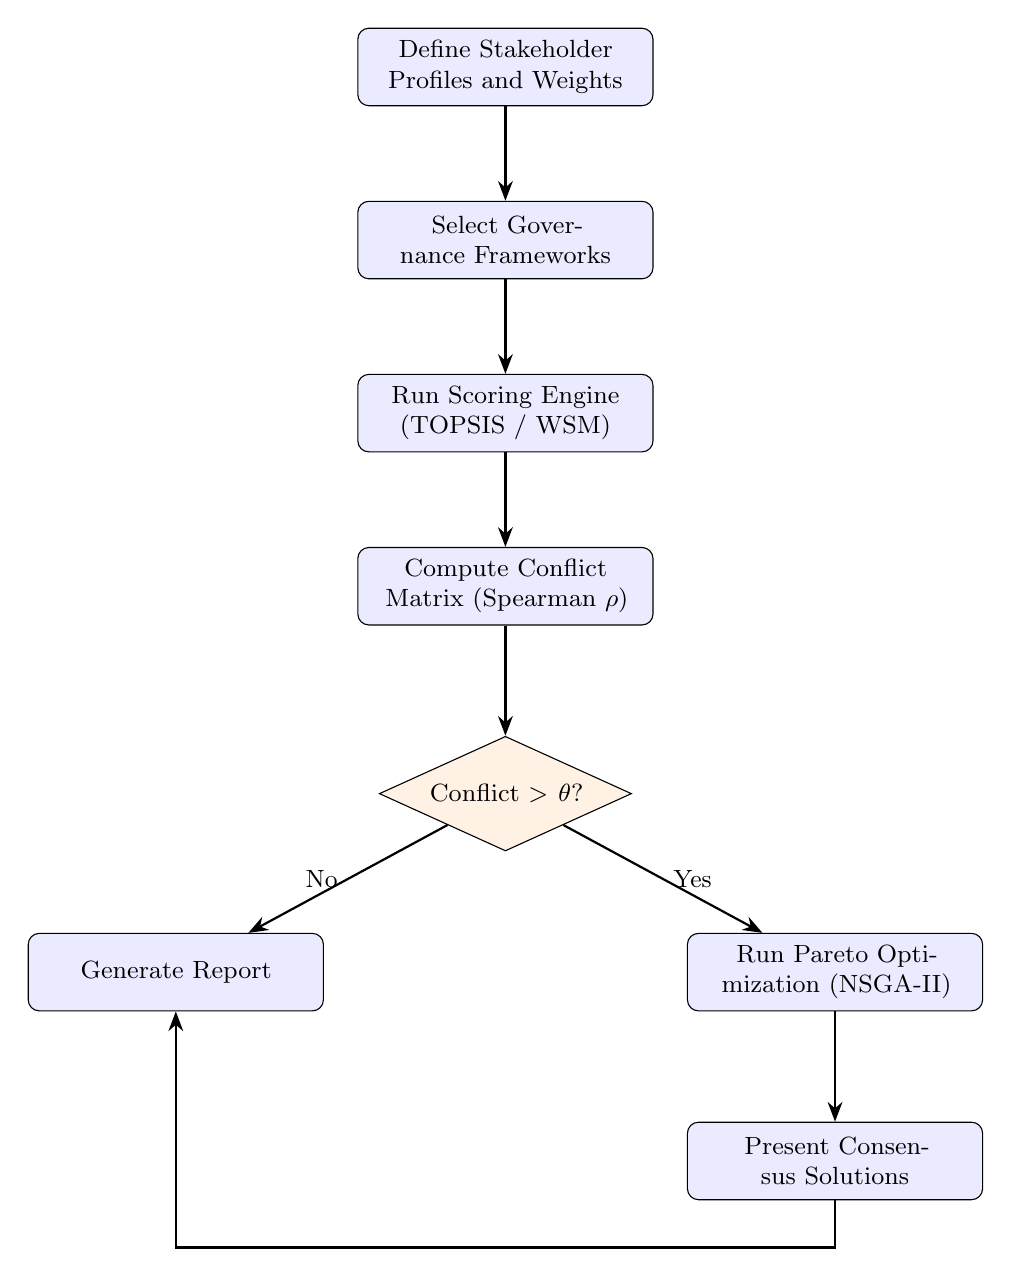
\begin{tikzpicture}[
  node distance=1.2cm and 1.5cm,
  block/.style={rectangle, draw, fill=blue!8, text width=10em, text centered, rounded corners, minimum height=2.8em, font=\small},
  decision/.style={diamond, draw, fill=orange!10, text width=7em, text centered, aspect=2.2, inner sep=1pt, font=\small},
  arrow/.style={-{Stealth[length=2.5mm]}, thick},
]
  \node[block] (define) {Define Stakeholder Profiles and Weights};
  \node[block, below=of define] (select) {Select Governance Frameworks};
  \node[block, below=of select] (score) {Run Scoring Engine (TOPSIS / WSM)};
  \node[block, below=of score] (conflict) {Compute Conflict Matrix (Spearman $\rho$)};
  \node[decision, below=1.4cm of conflict] (check) {Conflict $> \theta$?};
  \node[block, below left=1.4cm and 1.5cm of check] (report) {Generate Report};
  \node[block, below right=1.4cm and 1.5cm of check] (pareto) {Run Pareto Optimization (NSGA-II)};
  \node[block, below=1.4cm of pareto] (consensus) {Present Consensus Solutions};

  \draw[arrow] (define) -- (select);
  \draw[arrow] (select) -- (score);
  \draw[arrow] (score) -- (conflict);
  \draw[arrow] (conflict) -- (check);
  \draw[arrow] (check) -- node[left, font=\small] {No} (report);
  \draw[arrow] (check) -- node[right, font=\small] {Yes} (pareto);
  \draw[arrow] (pareto) -- (consensus);
  \draw[arrow] (consensus.south) -- ++(0,-0.6) -| (report.south);
\end{tikzpicture}
\caption{Stakeholder decision flow in MEDF.}
\label{fig:stakeholder_flow}
\end{figure}

This structured workflow ensures that the ethical evaluation is comprehensive, transparent, and grounded in a defensible methodology, transforming abstract ethical debates into a concrete, data-driven decision-making process.

\chapter{System Architecture}
\label{ch:architecture}

The MEDF platform is implemented as a modern web application with a clear separation of concerns, following a three-tier architecture. This design ensures modularity, scalability, and maintainability. The three primary layers are the Presentation Layer, the API/Orchestration Layer, and the Data/Configuration Layer. This chapter details the components within each layer and the interactions between them, as illustrated in Figure~\ref{fig:architecture}.

\begin{figure}[H]
\centering
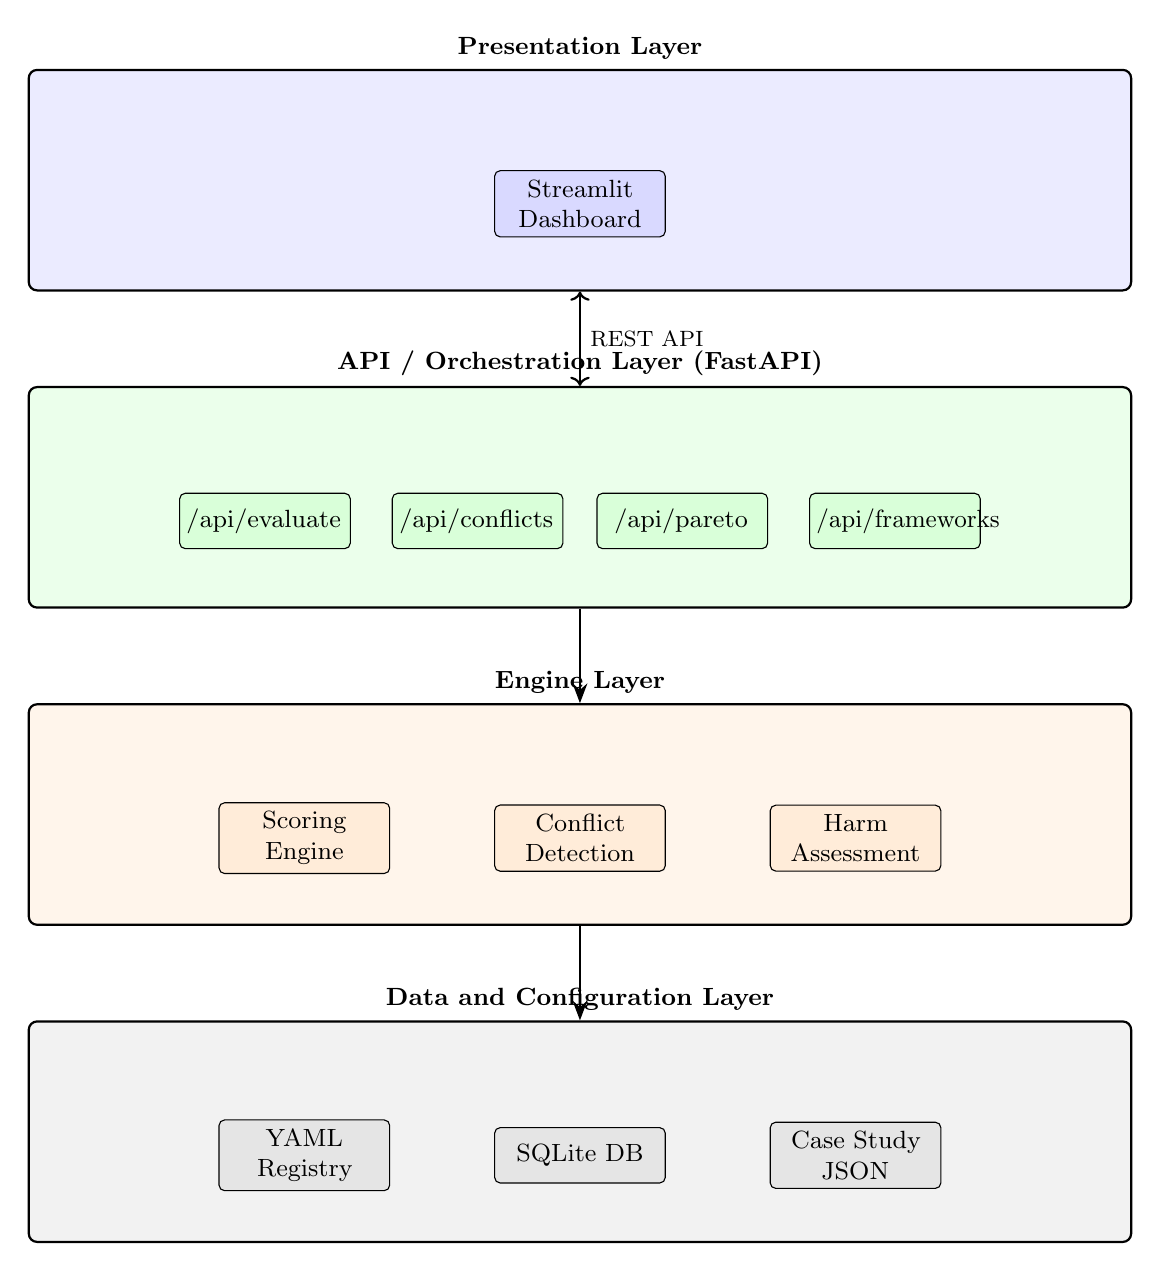
\begin{tikzpicture}[
  node distance=0.6cm,
  layer/.style={rectangle, draw, thick, minimum width=14cm, minimum height=2.8cm, rounded corners=3pt},
  comp/.style={rectangle, draw, fill=white, text width=5.5em, text centered, minimum height=2em, font=\small, rounded corners=2pt},
  arrow/.style={-{Stealth[length=2.5mm]}, thick},
]
  % Presentation Layer
  \node[layer, fill=blue!8] (pres) {};
  \node[above=0pt of pres.north, anchor=south, font=\bfseries\small] {Presentation Layer};
  \node[comp, fill=blue!15] at ([yshift=-0.3cm]pres.center) (streamlit) {Streamlit Dashboard};

  % API Layer
  \node[layer, fill=green!8, below=1.2cm of pres] (api) {};
  \node[above=0pt of api.north, anchor=south, font=\bfseries\small] {API / Orchestration Layer (FastAPI)};
  \node[comp, fill=green!15] at ([xshift=-4cm, yshift=-0.3cm]api.center) (eval) {/api/evaluate};
  \node[comp, fill=green!15] at ([xshift=-1.3cm, yshift=-0.3cm]api.center) (conf) {/api/conflicts};
  \node[comp, fill=green!15] at ([xshift=1.3cm, yshift=-0.3cm]api.center) (par) {/api/pareto};
  \node[comp, fill=green!15] at ([xshift=4cm, yshift=-0.3cm]api.center) (fw) {/api/frameworks};

  % Engine Layer
  \node[layer, fill=orange!8, below=1.2cm of api] (eng) {};
  \node[above=0pt of eng.north, anchor=south, font=\bfseries\small] {Engine Layer};
  \node[comp, fill=orange!15] at ([xshift=-3.5cm, yshift=-0.3cm]eng.center) (scoring) {Scoring Engine};
  \node[comp, fill=orange!15] at ([xshift=0cm, yshift=-0.3cm]eng.center) (conflict) {Conflict Detection};
  \node[comp, fill=orange!15] at ([xshift=3.5cm, yshift=-0.3cm]eng.center) (harm) {Harm Assessment};

  % Data Layer
  \node[layer, fill=gray!10, below=1.2cm of eng] (data) {};
  \node[above=0pt of data.north, anchor=south, font=\bfseries\small] {Data and Configuration Layer};
  \node[comp, fill=gray!20] at ([xshift=-3.5cm, yshift=-0.3cm]data.center) (yaml) {YAML Registry};
  \node[comp, fill=gray!20] at ([xshift=0cm, yshift=-0.3cm]data.center) (sqlite) {SQLite DB};
  \node[comp, fill=gray!20] at ([xshift=3.5cm, yshift=-0.3cm]data.center) (json) {Case Study JSON};

  % Arrows
  \draw[arrow, <->] (pres.south) -- node[right, font=\footnotesize] {REST API} (api.north);
  \draw[arrow] (api.south) -- (eng.north);
  \draw[arrow] (eng.south) -- (data.north);
\end{tikzpicture}
\caption{MEDF system architecture diagram.}
\label{fig:architecture}
\end{figure}

\section{Presentation Layer}
\label{sec:presentation}

The Presentation Layer is the user-facing component of the system, implemented as an interactive web dashboard using Streamlit. The complete frontend is contained within a single Python script, \texttt{streamlit\_app.py}. This choice was made to facilitate rapid prototyping and tight integration with the Python-based data analysis and visualization libraries used to display evaluation results.

The dashboard provides a graphical user interface (GUI) for analysts to:

\begin{itemize}[leftmargin=2em]
  \item Configure and initiate evaluation runs.
  \item Define or select AI systems and their baseline dimension scores.
  \item Select and customize stakeholder profiles and their priority weightings.
  \item View evaluation results, including overall scores, per-framework breakdowns, and dimensional contributions.
  \item Analyze stakeholder conflicts through correlation matrices and divergence tables.
  \item Trigger and explore Pareto-optimal consensus solutions.
  \item Export evaluation data and visualizations for reporting.
\end{itemize}

The Streamlit application communicates with the backend exclusively through the defined REST API, ensuring a clean separation between the user interface and the core business logic.

\section{API/Orchestration Layer}
\label{sec:api}

The backend is a robust API server built with FastAPI. FastAPI was chosen for its high performance, native support for asynchronous operations, and automatic generation of interactive OpenAPI documentation, which provides excellent visibility into the API contract for development and auditing. The API layer is responsible for orchestrating the complete evaluation workflow.

It is composed of several modular routers, each handling a specific domain of functionality:

\begin{itemize}[leftmargin=2em]
  \item \texttt{/api/frameworks}: Serves the definitions of the available governance frameworks.
  \item \texttt{/api/stakeholders}: Manages the creation, retrieval, and updating of stakeholder profiles.
  \item \texttt{/api/evaluate}: The primary endpoint for running an ethical evaluation. It receives the evaluation context and returns the computed scores.
  \item \texttt{/api/conflicts}: Analyzes the evaluation results to identify and quantify disagreements between stakeholders.
  \item \texttt{/api/pareto}: Executes the multi-objective optimization to find consensus solutions when conflicts are detected.
\end{itemize}

This layer acts as the central nervous system of the application, validating all incoming requests against strict Pydantic data models (\texttt{app/models.py}) and coordinating the execution of tasks by the Engine Layer.

\section{Engine Layer}
\label{sec:engine}

This layer contains the core algorithmic and business logic of the MEDF platform. It consists of several specialized Python modules:

\begin{itemize}[leftmargin=2em]
  \item \textbf{Scoring Engine} (\texttt{scoring\_engine.py}): Implements the MCDM algorithms, including TOPSIS and WSM, for calculating ethical scores.
  \item \textbf{Conflict Detection Stub} (\texttt{conflict\_detection.py}): Defines the interface contract for conflict analysis. In the current implementation, this module serves as a placeholder; all six of its public functions return empty or zero-valued results. The full conflict analysis logic---including Spearman's rank correlation, divergent-dimension identification, and harm-assessment integration---is implemented inline within \texttt{routers/conflicts.py}. A dedicated test (\texttt{test\_conflict\_detection\_placeholder\_contract.py}) verifies that the stub returns the expected empty results, confirming this architectural decision is intentional rather than accidental. Future refactoring may extract the inline logic into this module to complete the separation of concerns.
  \item \textbf{Harm Assessment} (\texttt{harm\_assessment.py}): Implements a model to estimate the potential severity of ethical risks. The harm score is computed as a weighted combination: $h = 0.7 \times (1 - s_{\text{norm}}) + 0.3 \times \bar{d}$, where $s_{\text{norm}}$ is the normalized dimension score and $\bar{d}$ is the mean pairwise stakeholder weight disagreement.
  \item \textbf{Pareto Engine} (\texttt{routers/pareto.py}): Integrates the NSGA-II algorithm via the \texttt{pymoo} library to compute the Pareto frontier of consensus weightings. A random-sampling fallback is provided if \texttt{pymoo} is unavailable.
\end{itemize}

These engines are stateless and operate on the data passed to them by the API layer, ensuring that the core logic is decoupled from the web-serving and data persistence concerns.

\section{Data and Configuration Layer}
\label{sec:data}

This layer is responsible for all data persistence and static configuration. It comprises:

\begin{itemize}[leftmargin=2em]
  \item \textbf{Framework YAML Registry.} The definitions for ALTAI, NIST RMF, and MGAF are stored in human-readable YAML files. This allows the governance criteria to be version-controlled and updated without changing application code. The \texttt{framework\_registry.py} module is responsible for loading and validating these files at startup.

  \item \textbf{SQLite Database.} A lightweight SQLite database is used to store stakeholder profiles. SQLAlchemy, a Python ORM, is used to interact with the database, providing an abstraction layer that would facilitate migration to a more powerful database system like PostgreSQL if needed.

  \item \textbf{Case Study JSON Files.} The three case studies are defined in structured JSON files, containing their baseline scores and contextual information. This allows for consistent and reproducible testing and demonstration.

  \item \textbf{Audit Logs.} To ensure complete traceability, the system can be configured to write detailed JSONL audit logs for every API request and response, capturing the exact inputs and outputs of every evaluation.
\end{itemize}

This layered architecture, summarized in the module diagram in Figure~\ref{fig:modules}, creates a robust and maintainable system where each component has a clearly defined responsibility.

\begin{figure}[H]
\centering
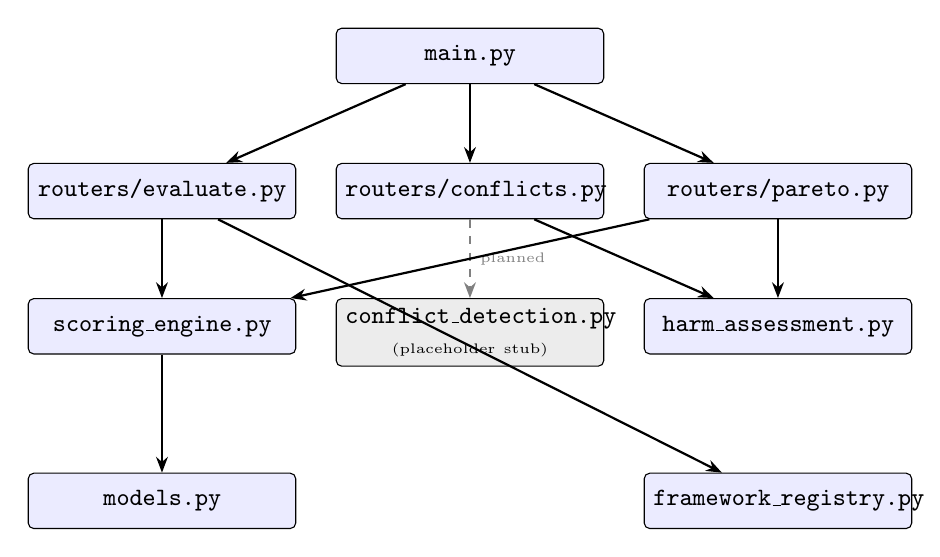
\begin{tikzpicture}[
  node distance=0.5cm and 0.8cm,
  mod/.style={rectangle, draw, fill=blue!8, text width=9em, text centered, minimum height=2em, font=\small, rounded corners=2pt},
  arrow/.style={-{Stealth[length=2mm]}, thick},
]
  \node[mod] (main) {\texttt{main.py}};
  \node[mod, below left=1cm and 0.5cm of main] (eval_r) {\texttt{routers/evaluate.py}};
  \node[mod, below=1cm of main] (conf_r) {\texttt{routers/conflicts.py}};
  \node[mod, below right=1cm and 0.5cm of main] (par_r) {\texttt{routers/pareto.py}};

  \node[mod, below=1cm of eval_r] (scoring) {\texttt{scoring\_engine.py}};
  \node[mod, fill=gray!15, below=1cm of conf_r] (conflict) {\texttt{conflict\_detection.py}\\{\tiny (placeholder stub)}};
  \node[mod, below=1cm of par_r] (harm) {\texttt{harm\_assessment.py}};

  \node[mod, below=1.5cm of scoring] (models) {\texttt{models.py}};
  \node[mod, below=1.5cm of harm] (registry) {\texttt{framework\_registry.py}};

  \draw[arrow] (main) -- (eval_r);
  \draw[arrow] (main) -- (conf_r);
  \draw[arrow] (main) -- (par_r);
  \draw[arrow] (eval_r) -- (scoring);
  \draw[arrow, dashed, gray] (conf_r) -- node[right, font=\tiny, text=gray] {planned} (conflict);
  \draw[arrow] (conf_r) -- (harm);
  \draw[arrow] (par_r) -- (harm);
  \draw[arrow] (scoring) -- (models);
  \draw[arrow] (eval_r) -- (registry);
  \draw[arrow] (par_r) -- (scoring);
\end{tikzpicture}
\caption{MEDF software module diagram.}
\label{fig:modules}
\end{figure}

\chapter{Algorithm Design}
\label{ch:algorithms}

The analytical power of the MEDF platform is derived from a set of carefully selected and implemented algorithms that translate qualitative ethical considerations into a quantitative, decision-oriented format. This chapter details the design of the core algorithms responsible for scoring, weighting, and conflict resolution.

\section{Ethical Scoring Engine}
\label{sec:scoring_engine}

The scoring engine is the heart of the evaluation pipeline. Its purpose is to compute a single, normalized score representing the ethical performance of an AI system, taking into account the system's characteristics, the chosen governance framework, and the priorities of a given stakeholder. This process involves three steps: weighting, aggregation, and normalization.

\subsection{Stakeholder and Framework Weighting}
\label{sec:weighting}

The evaluation process begins by establishing the \enquote{effective weights} for each of the six Unified Dimensions. This is not simply the stakeholder's stated priorities. Instead, MEDF computes a combined weight that reflects both the stakeholder's values and the intrinsic emphasis of the selected governance framework. This is achieved through a \textbf{product pooling method}:

\begin{enumerate}[leftmargin=2em]
  \item \textbf{Stakeholder Weights} ($\mathbf{w}_s$): Each stakeholder provides a vector of weights, where each element represents the importance they assign to a dimension. This vector is normalized to sum to 1.0.

  \item \textbf{Framework Weights} ($\mathbf{w}_f$): For each governance framework, a vector of intrinsic weights is pre-calculated. This is derived from the structure of the framework itself, for example, by counting the number of requirements, clauses, or principles related to each dimension. This vector is also normalized to sum to 1.0.

  \item \textbf{Effective Weights} ($\mathbf{w}_{\mathrm{eff}}$): The effective weight for each dimension is calculated as the element-wise product of the stakeholder and framework weight vectors. The resulting vector is then re-normalized to sum to 1.0:
\end{enumerate}

\begin{equation}
  \mathbf{w}_{\mathrm{eff}} \propto \mathbf{w}_s \odot \mathbf{w}_f
  \label{eq:effective_weights}
\end{equation}

This product pooling approach ensures that a dimension receives a high effective weight only if \textit{both} the stakeholder and the framework consider it important. A dimension that is critical to the stakeholder but not emphasized by the framework (or vice versa) will receive a moderate effective weight. This prevents any single source of weighting from dominating the evaluation and produces a more balanced, context-sensitive result.

\subsection{TOPSIS for Score Aggregation}
\label{sec:topsis_algo}

TOPSIS (Technique for Order of Preference by Similarity to Ideal Solution)~\cite{hwang1981mcdm,behzadian2012topsis} is the primary scoring method in MEDF. Given a decision matrix $\mathbf{D}$ containing the AI system's scores across the six dimensions and the effective weight vector $\mathbf{w}_{\mathrm{eff}}$, the TOPSIS algorithm proceeds as follows:

\textbf{Step 1: Normalize the Decision Matrix.} Raw Likert scores (1--7) are scaled to the $[0, 1]$ range:
\begin{equation}
  x'_{ij} = \frac{x_{ij} - 1}{7 - 1}
  \label{eq:normalize}
\end{equation}

\textbf{Step 2: Vector Normalization.} The scaled matrix is then vector-normalized:
\begin{equation}
  r_{ij} = \frac{x'_{ij}}{\sqrt{\sum_{i} (x'_{ij})^2}}
  \label{eq:vector_norm}
\end{equation}

\textbf{Step 3: Weighted Normalized Matrix.} The normalized values are multiplied by the effective weights:
\begin{equation}
  v_{ij} = r_{ij} \times w_{\mathrm{eff},j}
  \label{eq:weighted}
\end{equation}

\textbf{Step 4: Determine Ideal and Anti-Ideal Solutions.} For benefit criteria (where higher is better), the ideal solution $A^+$ contains the maximum values and the anti-ideal solution $A^-$ contains the minimum values:
\begin{equation}
  A^+ = \{\max(v_{ij})\}, \quad A^- = \{\min(v_{ij})\}
  \label{eq:ideal}
\end{equation}

\textbf{Step 5: Calculate Euclidean Distances.} The distance of each alternative to the ideal and anti-ideal solutions is computed:
\begin{equation}
  d^+ = \sqrt{\sum_{j} (v_{ij} - A^+_j)^2}, \quad d^- = \sqrt{\sum_{j} (v_{ij} - A^-_j)^2}
  \label{eq:distances}
\end{equation}

\textbf{Step 6: Closeness Coefficient.} The final TOPSIS score is the closeness coefficient:
\begin{equation}
  C = \frac{d^-}{d^+ + d^-}
  \label{eq:closeness}
\end{equation}

A score of $C = 1.0$ indicates a perfect match with the ideal solution, while $C = 0.0$ indicates a match with the anti-ideal solution. The scoring aggregation process is illustrated in Figure~\ref{fig:scoring_flow}.

\begin{figure}[H]
\centering
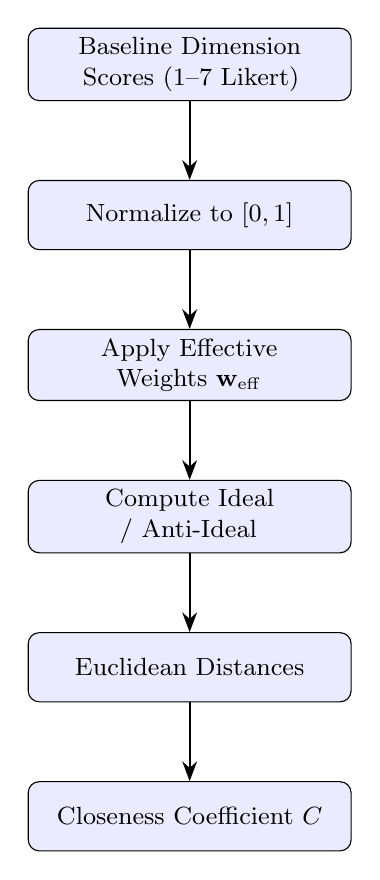
\begin{tikzpicture}[
  node distance=1cm,
  block/.style={rectangle, draw, fill=blue!8, text width=11em, text centered, rounded corners, minimum height=2.5em, font=\small},
  arrow/.style={-{Stealth[length=2.5mm]}, thick},
]
  \node[block] (input) {Baseline Dimension Scores (1--7 Likert)};
  \node[block, below=of input] (norm) {Normalize to $[0,1]$};
  \node[block, below=of norm] (weight) {Apply Effective Weights $\mathbf{w}_{\mathrm{eff}}$};
  \node[block, below=of weight] (ideal) {Compute Ideal / Anti-Ideal};
  \node[block, below=of ideal] (dist) {Euclidean Distances};
  \node[block, below=of dist] (score) {Closeness Coefficient $C$};

  \draw[arrow] (input) -- (norm);
  \draw[arrow] (norm) -- (weight);
  \draw[arrow] (weight) -- (ideal);
  \draw[arrow] (ideal) -- (dist);
  \draw[arrow] (dist) -- (score);
\end{tikzpicture}
\caption{Ethical scoring aggregation process.}
\label{fig:scoring_flow}
\end{figure}

\section{Conflict Detection and Consensus Generation}
\label{sec:conflict}

\subsection{Conflict Detection with Spearman's Correlation}
\label{sec:spearman}

To quantify the degree of agreement or disagreement between stakeholder groups, MEDF uses Spearman's rank correlation coefficient ($\rho$). For each pair of stakeholders, the algorithm computes the correlation between their weight vectors. A $\rho$ close to $+1$ indicates strong agreement (both stakeholders rank the dimensions in a similar order of importance), while a $\rho$ close to $-1$ indicates strong disagreement (their priorities are inversely related). A $\rho$ near $0$ indicates no significant relationship.

The conflict detection module computes two types of correlation matrices:

\begin{enumerate}[leftmargin=2em]
  \item \textbf{Priority Conflict (Weights-Only).} This matrix computes Spearman's $\rho$ directly between the raw stakeholder weight vectors. It measures whether stakeholders agree on which dimensions are most important, independent of the AI system being evaluated.

  \item \textbf{System-Salience Conflict (Contribution-Based).} This matrix computes Spearman's $\rho$ between the \enquote{contribution vectors}, which are the element-wise products of the effective weights and the system's dimension scores. This measures whether stakeholders agree on which dimensions contribute most to the final score for a specific AI system. Two stakeholders might disagree on general priorities but agree on the critical issues for a particular system.
\end{enumerate}

\subsection{Pareto Optimization with NSGA-II}
\label{sec:pareto}

When the conflict analysis reveals significant disagreement between stakeholders, MEDF employs the NSGA-II algorithm~\cite{deb2002nsga2} to find a set of Pareto-optimal consensus weight vectors. The optimization problem is formulated as follows:

For each stakeholder $k$, define an objective function that measures the weighted distance between a candidate consensus weight vector $\mathbf{w}_c$ and the stakeholder's preferred weight vector $\mathbf{w}_k$:
\begin{equation}
  f_k(\mathbf{w}_c) = \sum_{i} s_i \cdot |w_{c,i} - w_{k,i}|
  \label{eq:pareto_obj}
\end{equation}
where $s_i$ is a salience factor derived from the AI system's dimension scores, ensuring that the optimization prioritizes agreement on the dimensions that matter most for the system under evaluation.

NSGA-II then searches for the set of weight vectors that minimize all objective functions simultaneously. The resulting Pareto frontier represents the set of all possible compromises where no stakeholder can be made better off without making another worse off. Each point on the frontier is a viable consensus solution, and the decision-makers can select the one that best reflects the desired balance of interests.

\section{Weighted Sum Model (WSM)}
\label{sec:wsm}

In addition to TOPSIS, MEDF implements the Weighted Sum Model (WSM) as an alternative scoring method. WSM computes the overall score as a simple weighted average of the normalized dimension scores:
\begin{equation}
  S_{\mathrm{WSM}} = \sum_{j} w_{\mathrm{eff},j} \times x'_j
  \label{eq:wsm}
\end{equation}
WSM is simpler and more intuitive than TOPSIS but does not account for the distance to ideal and anti-ideal solutions. It is provided as an option for users who prefer a more straightforward aggregation method or who wish to compare results across different scoring approaches.

\section{Harm Assessment Model}
\label{sec:harm}

The harm assessment module provides a high-level risk classification based on the evaluation results. It maps the overall score to a risk level using predefined thresholds:

\begin{table}[H]
\centering
\caption{Risk classification thresholds.}
\label{tab:risk_levels}
\begin{tabular}{@{}lll@{}}
\toprule
\textbf{Score Range} & \textbf{Risk Level} & \textbf{Description} \\
\midrule
0.00--0.25 & Critical & Severe ethical deficiencies. \\
0.25--0.50 & High & Significant ethical concerns. \\
0.50--0.75 & Medium & Moderate ethical issues. \\
0.75--1.00 & Low & Acceptable ethical performance. \\
\bottomrule
\end{tabular}
\end{table}

The harm assessment also considers the level of stakeholder conflict. A system with a moderate overall score but high stakeholder conflict may be flagged as higher risk than its score alone would suggest, reflecting the additional governance challenge posed by unresolved ethical disagreements.

\section{End-to-End Evaluation Pipeline}
\label{sec:pipeline}

The complete MEDF evaluation pipeline integrates all the components described above into a coherent, sequential workflow. Figure~\ref{fig:pipeline} illustrates the end-to-end process from input to output.

\begin{figure}[H]
\centering
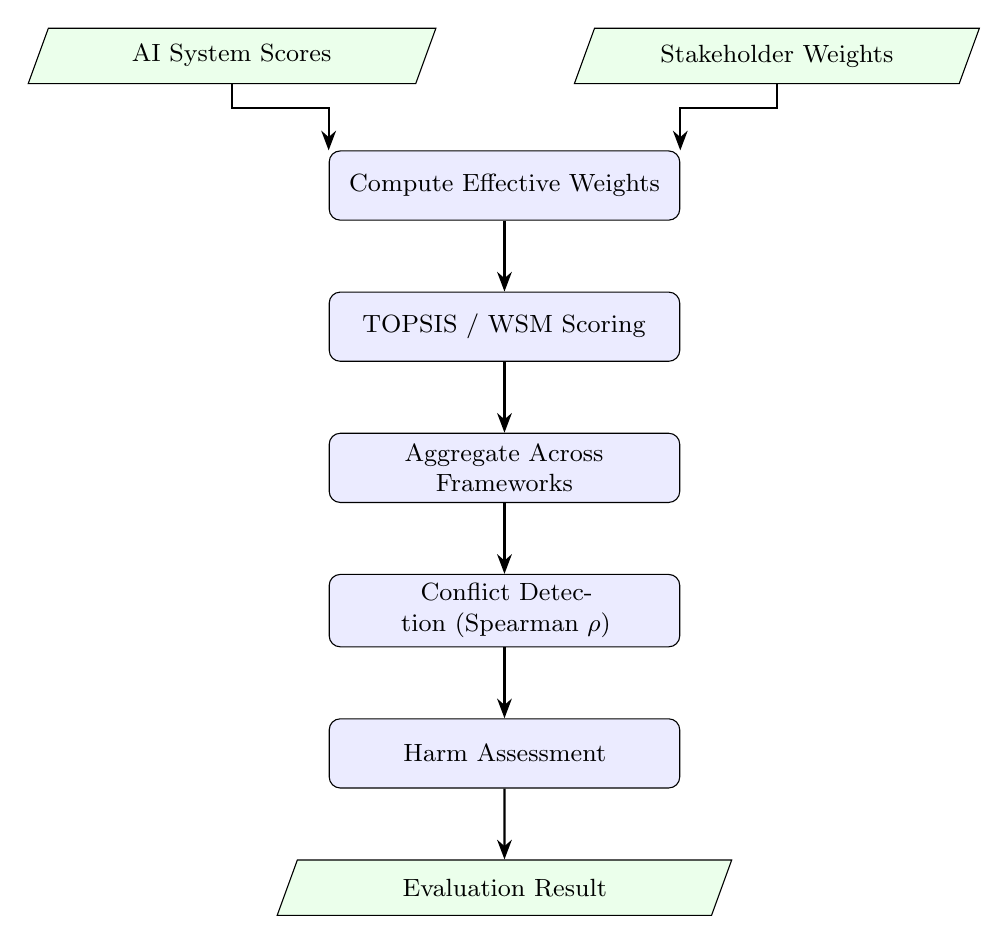
\begin{tikzpicture}[
  node distance=0.9cm,
  block/.style={rectangle, draw, fill=blue!8, text width=12em, text centered, rounded corners, minimum height=2.5em, font=\small},
  io/.style={trapezium, draw, fill=green!8, trapezium left angle=70, trapezium right angle=110, text width=9em, text centered, minimum height=2em, font=\small},
  arrow/.style={-{Stealth[length=2.5mm]}, thick},
]
  \node[io] (in1) {AI System Scores};
  \node[io, right=2cm of in1] (in2) {Stakeholder Weights};
  \node[block, below=1.2cm of $(in1)!0.5!(in2)$] (ew) {Compute Effective Weights};
  \node[block, below=of ew] (topsis) {TOPSIS / WSM Scoring};
  \node[block, below=of topsis] (agg) {Aggregate Across Frameworks};
  \node[block, below=of agg] (conflict) {Conflict Detection (Spearman $\rho$)};
  \node[block, below=of conflict] (harm) {Harm Assessment};
  \node[io, below=of harm] (out) {Evaluation Result};

  \draw[arrow] (in1.south) -- ++(0,-0.3) -| (ew.north west);
  \draw[arrow] (in2.south) -- ++(0,-0.3) -| (ew.north east);
  \draw[arrow] (ew) -- (topsis);
  \draw[arrow] (topsis) -- (agg);
  \draw[arrow] (agg) -- (conflict);
  \draw[arrow] (conflict) -- (harm);
  \draw[arrow] (harm) -- (out);
\end{tikzpicture}
\caption{End-to-end MEDF evaluation pipeline.}
\label{fig:pipeline}
\end{figure}

\chapter{Implementation}
\label{ch:implementation}

This chapter details the technical implementation of the MEDF platform, translating the architectural and algorithmic design into a concrete software artifact. The implementation is based on a modern Python technology stack and emphasizes code quality, testability, and reproducibility. The complete source code is available in the accompanying GitHub repository.

\section{Technology Stack}
\label{sec:tech_stack}

The project uses a curated set of open-source libraries and frameworks:

\begin{itemize}[leftmargin=2em]
  \item \textbf{Backend Framework.} FastAPI is used for the API server, providing a high-performance, asynchronous foundation with excellent data validation capabilities through its integration with Pydantic.

  \item \textbf{Frontend Framework.} Streamlit is used for the interactive web dashboard, enabling rapid development of data-centric user interfaces directly in Python.

  \item \textbf{Data Persistence.} SQLAlchemy serves as the Object-Relational Mapper (ORM) for interacting with a simple SQLite database. This choice prioritizes ease of setup and reproducibility for a research prototype, while the ORM provides a clear path for future migration to a more robust database.

  \item \textbf{Numerical and Scientific Computing.} NumPy is used for all numerical operations, particularly in the scoring and conflict detection engines, providing efficient and reliable array computations. The \texttt{pymoo} library is used for the implementation of the NSGA-II algorithm.

  \item \textbf{Configuration.} Framework definitions are managed using YAML, a human-readable data serialization format, which allows for easy editing and versioning of governance criteria.

  \item \textbf{Testing.} Pytest is used as the testing framework, with a comprehensive suite of over 50 tests covering unit, integration, property-based, and end-to-end scenarios.
\end{itemize}

\section{Codebase Structure and Critical Modules}
\label{sec:codebase}

The repository is organized into several distinct directories, reflecting the modular architecture. The core application logic resides in the \texttt{app/} directory.

\subsection{\texttt{app/main.py}}

This is the main entry point for the FastAPI application. It is responsible for initializing the application, setting up the database connection, loading the framework definitions from the YAML registry at startup, and including the API routers.

\subsection{\texttt{app/models.py}}

This module contains all the Pydantic data models that define the API schemas for requests and responses. It also includes the SQLAlchemy ORM models for the database tables (e.g., \texttt{DBStakeholderProfile}). This strict, centralized schema definition is critical for ensuring data consistency and providing clear API contracts.

\subsection{\texttt{app/scoring\_engine.py}}

This module contains the core algorithmic implementation for the scoring process. It includes functions for Likert score normalization, weight validation, and the implementations of the TOPSIS and WSM scoring methods. The code is written using NumPy for efficient vector and matrix operations.

\subsection{\texttt{app/routers/}}

The \texttt{app/routers/} directory contains the individual FastAPI routers for each major API endpoint:

\begin{itemize}[leftmargin=2em]
  \item \texttt{evaluate.py} handles the \texttt{/api/evaluate} endpoint. It receives the \texttt{EvaluateRequest} payload, computes effective weights through section-based product pooling of stakeholder and framework weights, coordinates calls to the scoring engine, and returns a validated \texttt{EvaluationResult} response.

  \item \texttt{conflicts.py} handles the \texttt{/api/conflicts} endpoint and is the \emph{de facto} conflict analysis engine. It implements the complete Spearman rank correlation computation for both weights-only and contribution-based conflict metrics, identifies divergent dimensions, determines conflict severity levels, and integrates the harm assessment module. As noted in Chapter~\ref{ch:architecture}, this logic currently remains in the router layer rather than an extracted standalone engine module.

  \item \texttt{pareto.py} handles the \texttt{/api/pareto} endpoint and implements the NSGA-II multi-objective optimization for computing Pareto-optimal consensus weight vectors.
\end{itemize}

This modular approach keeps the endpoint logic clean and organized, though the concentration of conflict analysis logic within the router rather than a dedicated engine module is an acknowledged technical debt item.

\section{Design Decisions and Implementation Rationale}
\label{sec:decisions}

A critical aspect of the implementation process was making deliberate engineering decisions to balance rigor, reproducibility, and development velocity. These decisions are documented in \texttt{docs/design\_decisions.md}.

\begin{itemize}[leftmargin=2em]
  \item \textbf{Why Weighted Scoring?} A simple unweighted average of dimension scores would fail to capture the differential importance of ethical criteria. Weighted scoring, where weights are explicitly defined by stakeholders and frameworks, provides a more nuanced and realistic evaluation model.

  \item \textbf{Why Configurable Stakeholder Weights?} Ethical priorities are subjective and context-dependent. Hardcoding a single set of weights would impose a single value system. Making weights configurable is the core mechanism that allows MEDF to model multi-stakeholder perspectives and surface conflicts.

  \item \textbf{Why a Sequential Evaluation Pipeline?} The evaluation pipeline (weighting, scoring, aggregation) is designed as a deterministic, sequential process. This ensures that the results are reproducible and the logic is easy to follow and audit. Parallelizing these steps would introduce unnecessary complexity without a clear benefit for this application.

  \item \textbf{Why a Three-Tier Architecture?} The separation of the presentation (Streamlit), API (FastAPI), and data layers creates a loosely coupled system. This allows each component to be developed, tested, and scaled independently. For example, the Streamlit frontend could be replaced with a React application without requiring any changes to the backend API.
\end{itemize}

\section{Reproducibility and Testing}
\label{sec:testing}

Ensuring the reproducibility of the research artifact was a primary implementation goal. This was achieved through several mechanisms:

\begin{itemize}[leftmargin=2em]
  \item \textbf{Dependency Pinning.} All Python dependencies are pinned to specific versions in \texttt{requirements.txt} to ensure a consistent runtime environment.

  \item \textbf{Deterministic Algorithms.} The core scoring algorithms are deterministic. The NSGA-II implementation uses a fixed random seed during evaluation runs to ensure that the Pareto frontier results are also reproducible.

  \item \textbf{Comprehensive Test Suite.} The Pytest suite includes tests that lock down the API contract (\texttt{test\_api\_contract\_lock.py}), verify the mathematical correctness of the scoring engine against hand-calculated examples (\texttt{test\_topsis\_hand\_verification.py}), and run end-to-end evaluations with the case study data to prevent regressions.

  \item \textbf{Continuous Integration.} GitHub Actions are configured to run the complete test suite on every push and pull request, ensuring that the codebase remains in a valid and tested state at all times.
\end{itemize}

This rigorous approach to implementation and testing ensures that MEDF is not just a conceptual framework, but a reliable and defensible software tool.

\chapter{Platform Interface}
\label{ch:interface}

The MEDF platform is equipped with an interactive web-based dashboard built using Streamlit. This interface provides a user-friendly environment for analysts, developers, and other stakeholders to conduct ethical evaluations without needing to interact directly with the backend API or the codebase. The dashboard is designed to guide the user through the evaluation workflow, from configuration to results analysis. This chapter describes the critical features and components of the user interface, illustrated with screenshots captured from the live application running on localhost.

\section{Main Evaluation View}
\label{sec:main_view}

The primary view lets the user configure and run a new evaluation by selecting an AI system, setting baseline dimension scores on the 1--7 Likert scale and choosing the frameworks and stakeholder profiles to include in the analysis. A \enquote{Run Demo Scenario} button populates the form with pre-configured case study data to support quick demonstration and testing. Figure~\ref{fig:evaluate_tab} shows the evaluation configuration interface.

\begin{figure}[H]
\centering
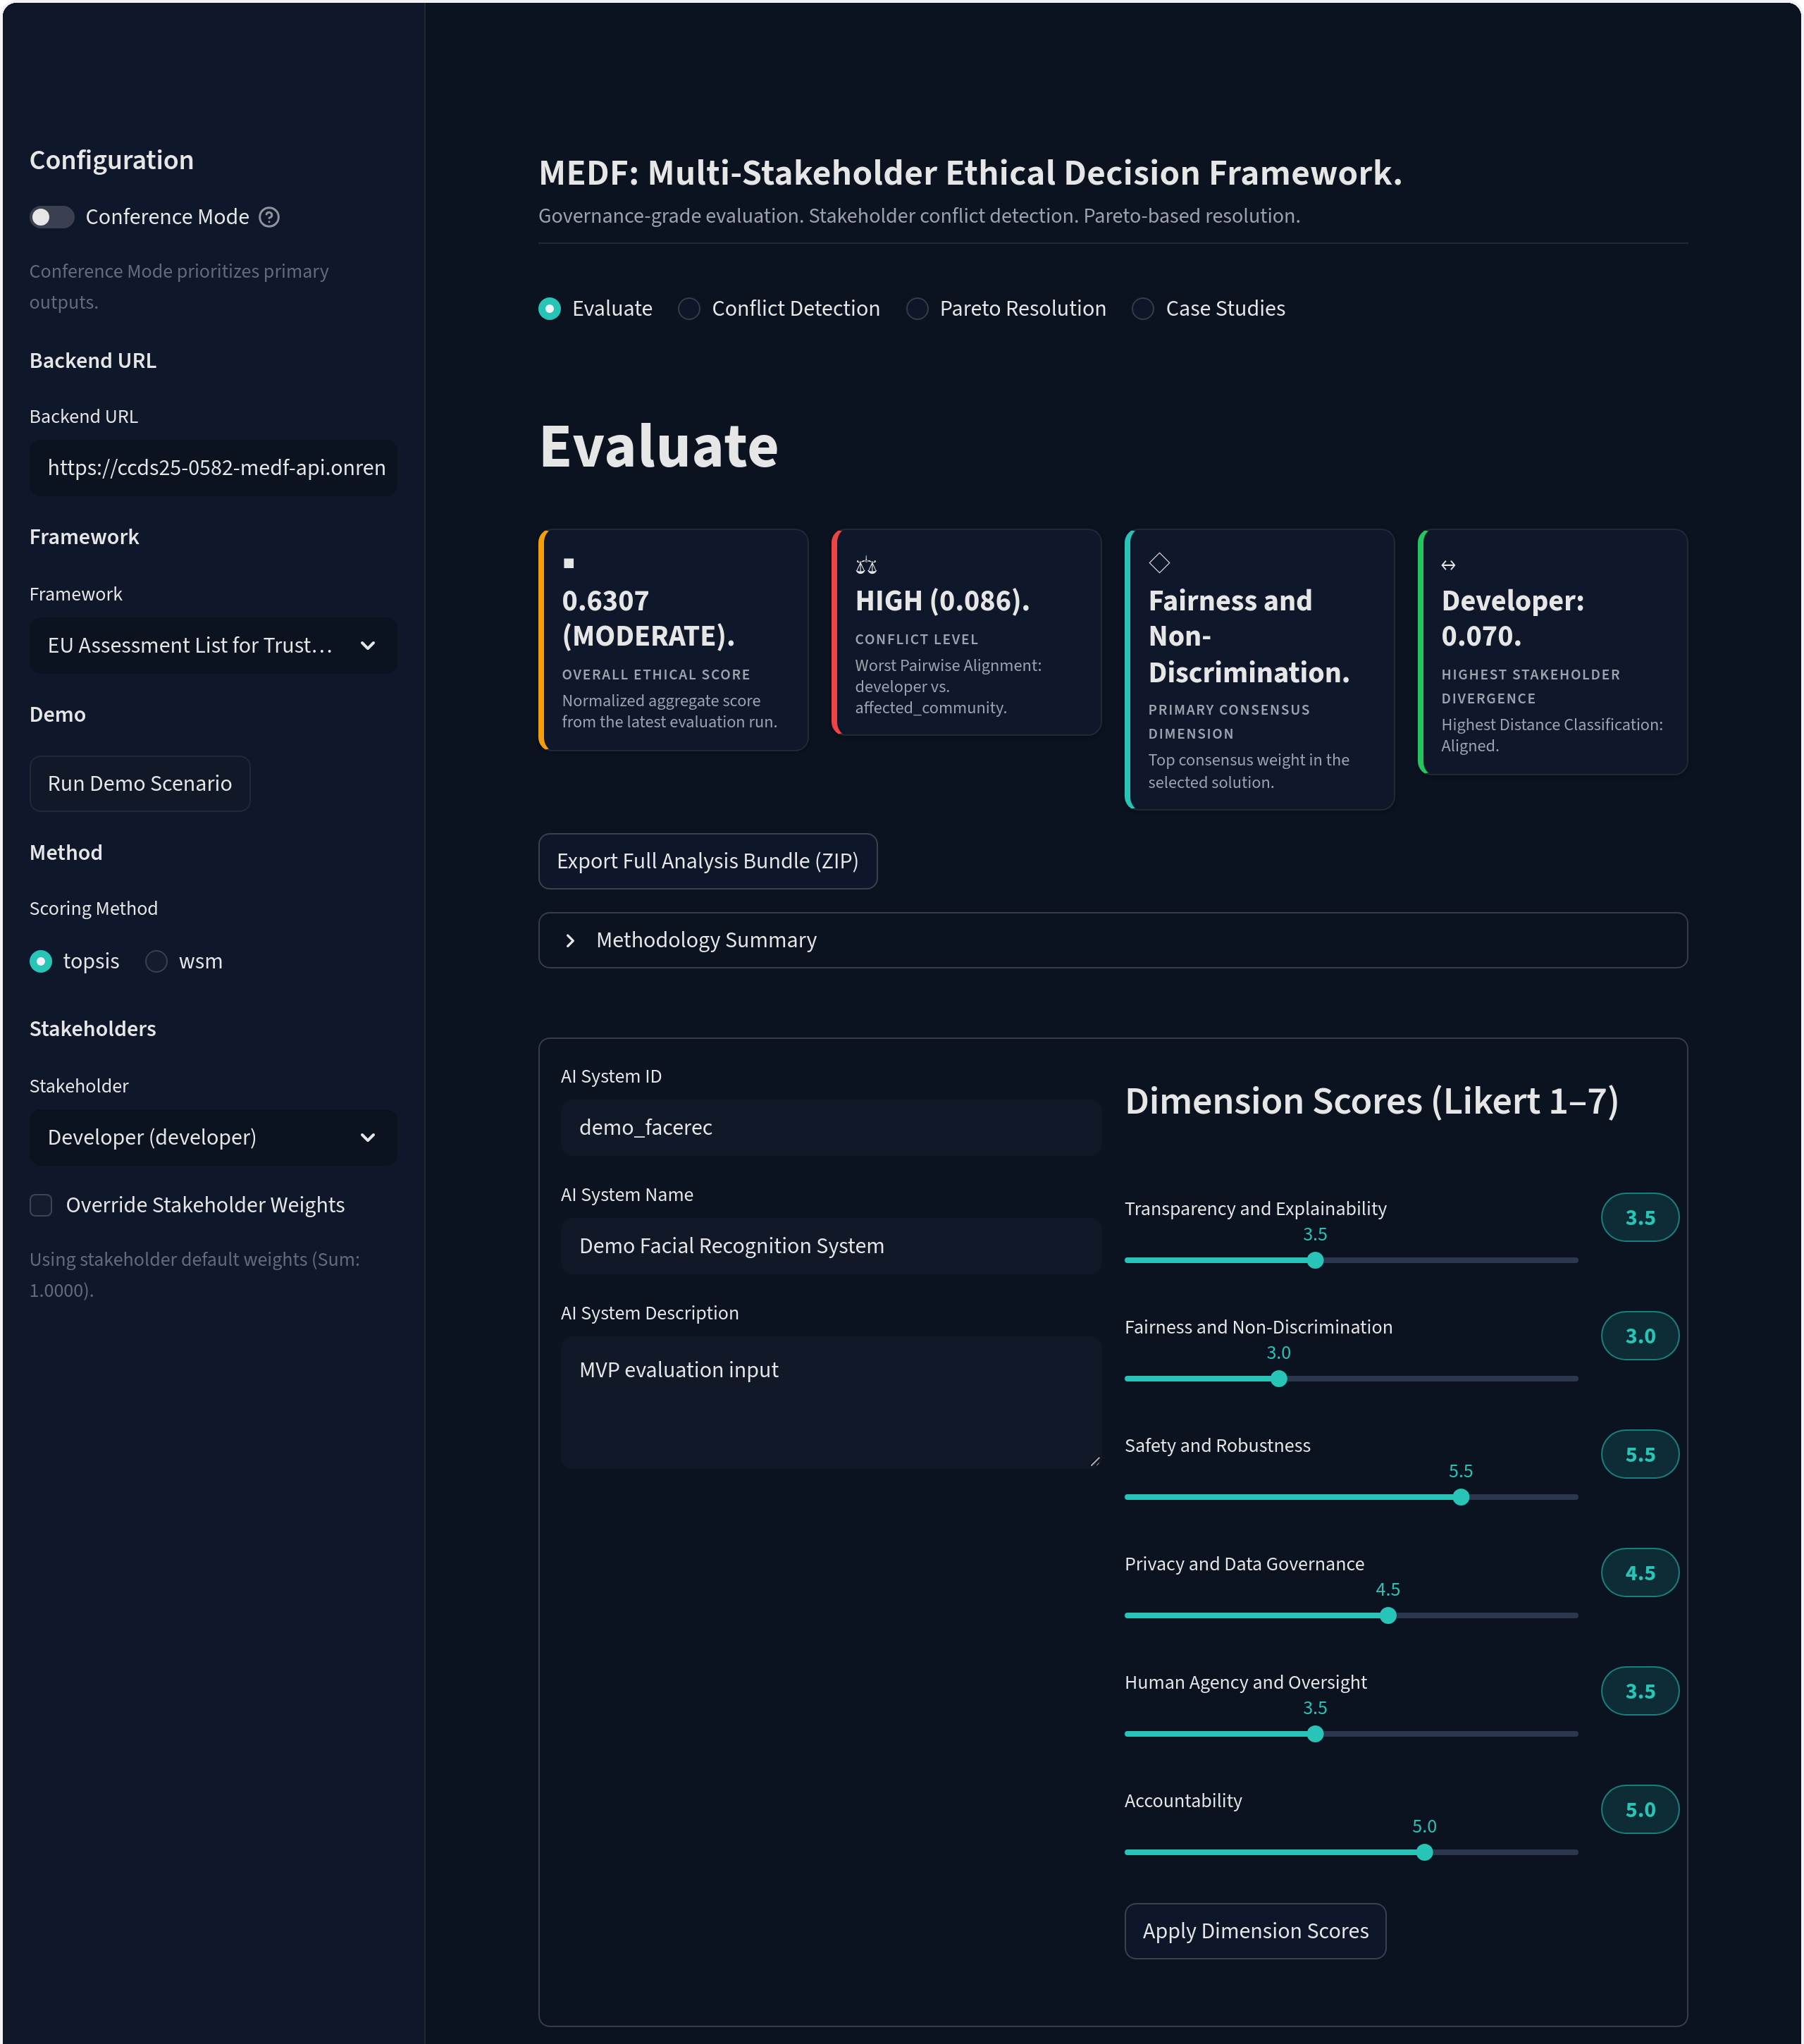
\includegraphics[width=0.95\textwidth]{figures/fig_10_1_evaluate_config.png}
\caption{MEDF evaluation configuration interface showing dimension score sliders, framework selection, and stakeholder weight customization.}
\label{fig:evaluate_tab}
\end{figure}

\section{Results Visualization}
\label{sec:results_viz}

Once an evaluation completes, the dashboard presents the outcome as an overall score gauge (color-coded by risk level), a framework score breakdown bar chart and a dimensional contribution radar chart that surfaces the ethical strengths and weaknesses of the system. Figure~\ref{fig:evaluate_results} shows the evaluation results after running the demo scenario.

\begin{figure}[H]
\centering
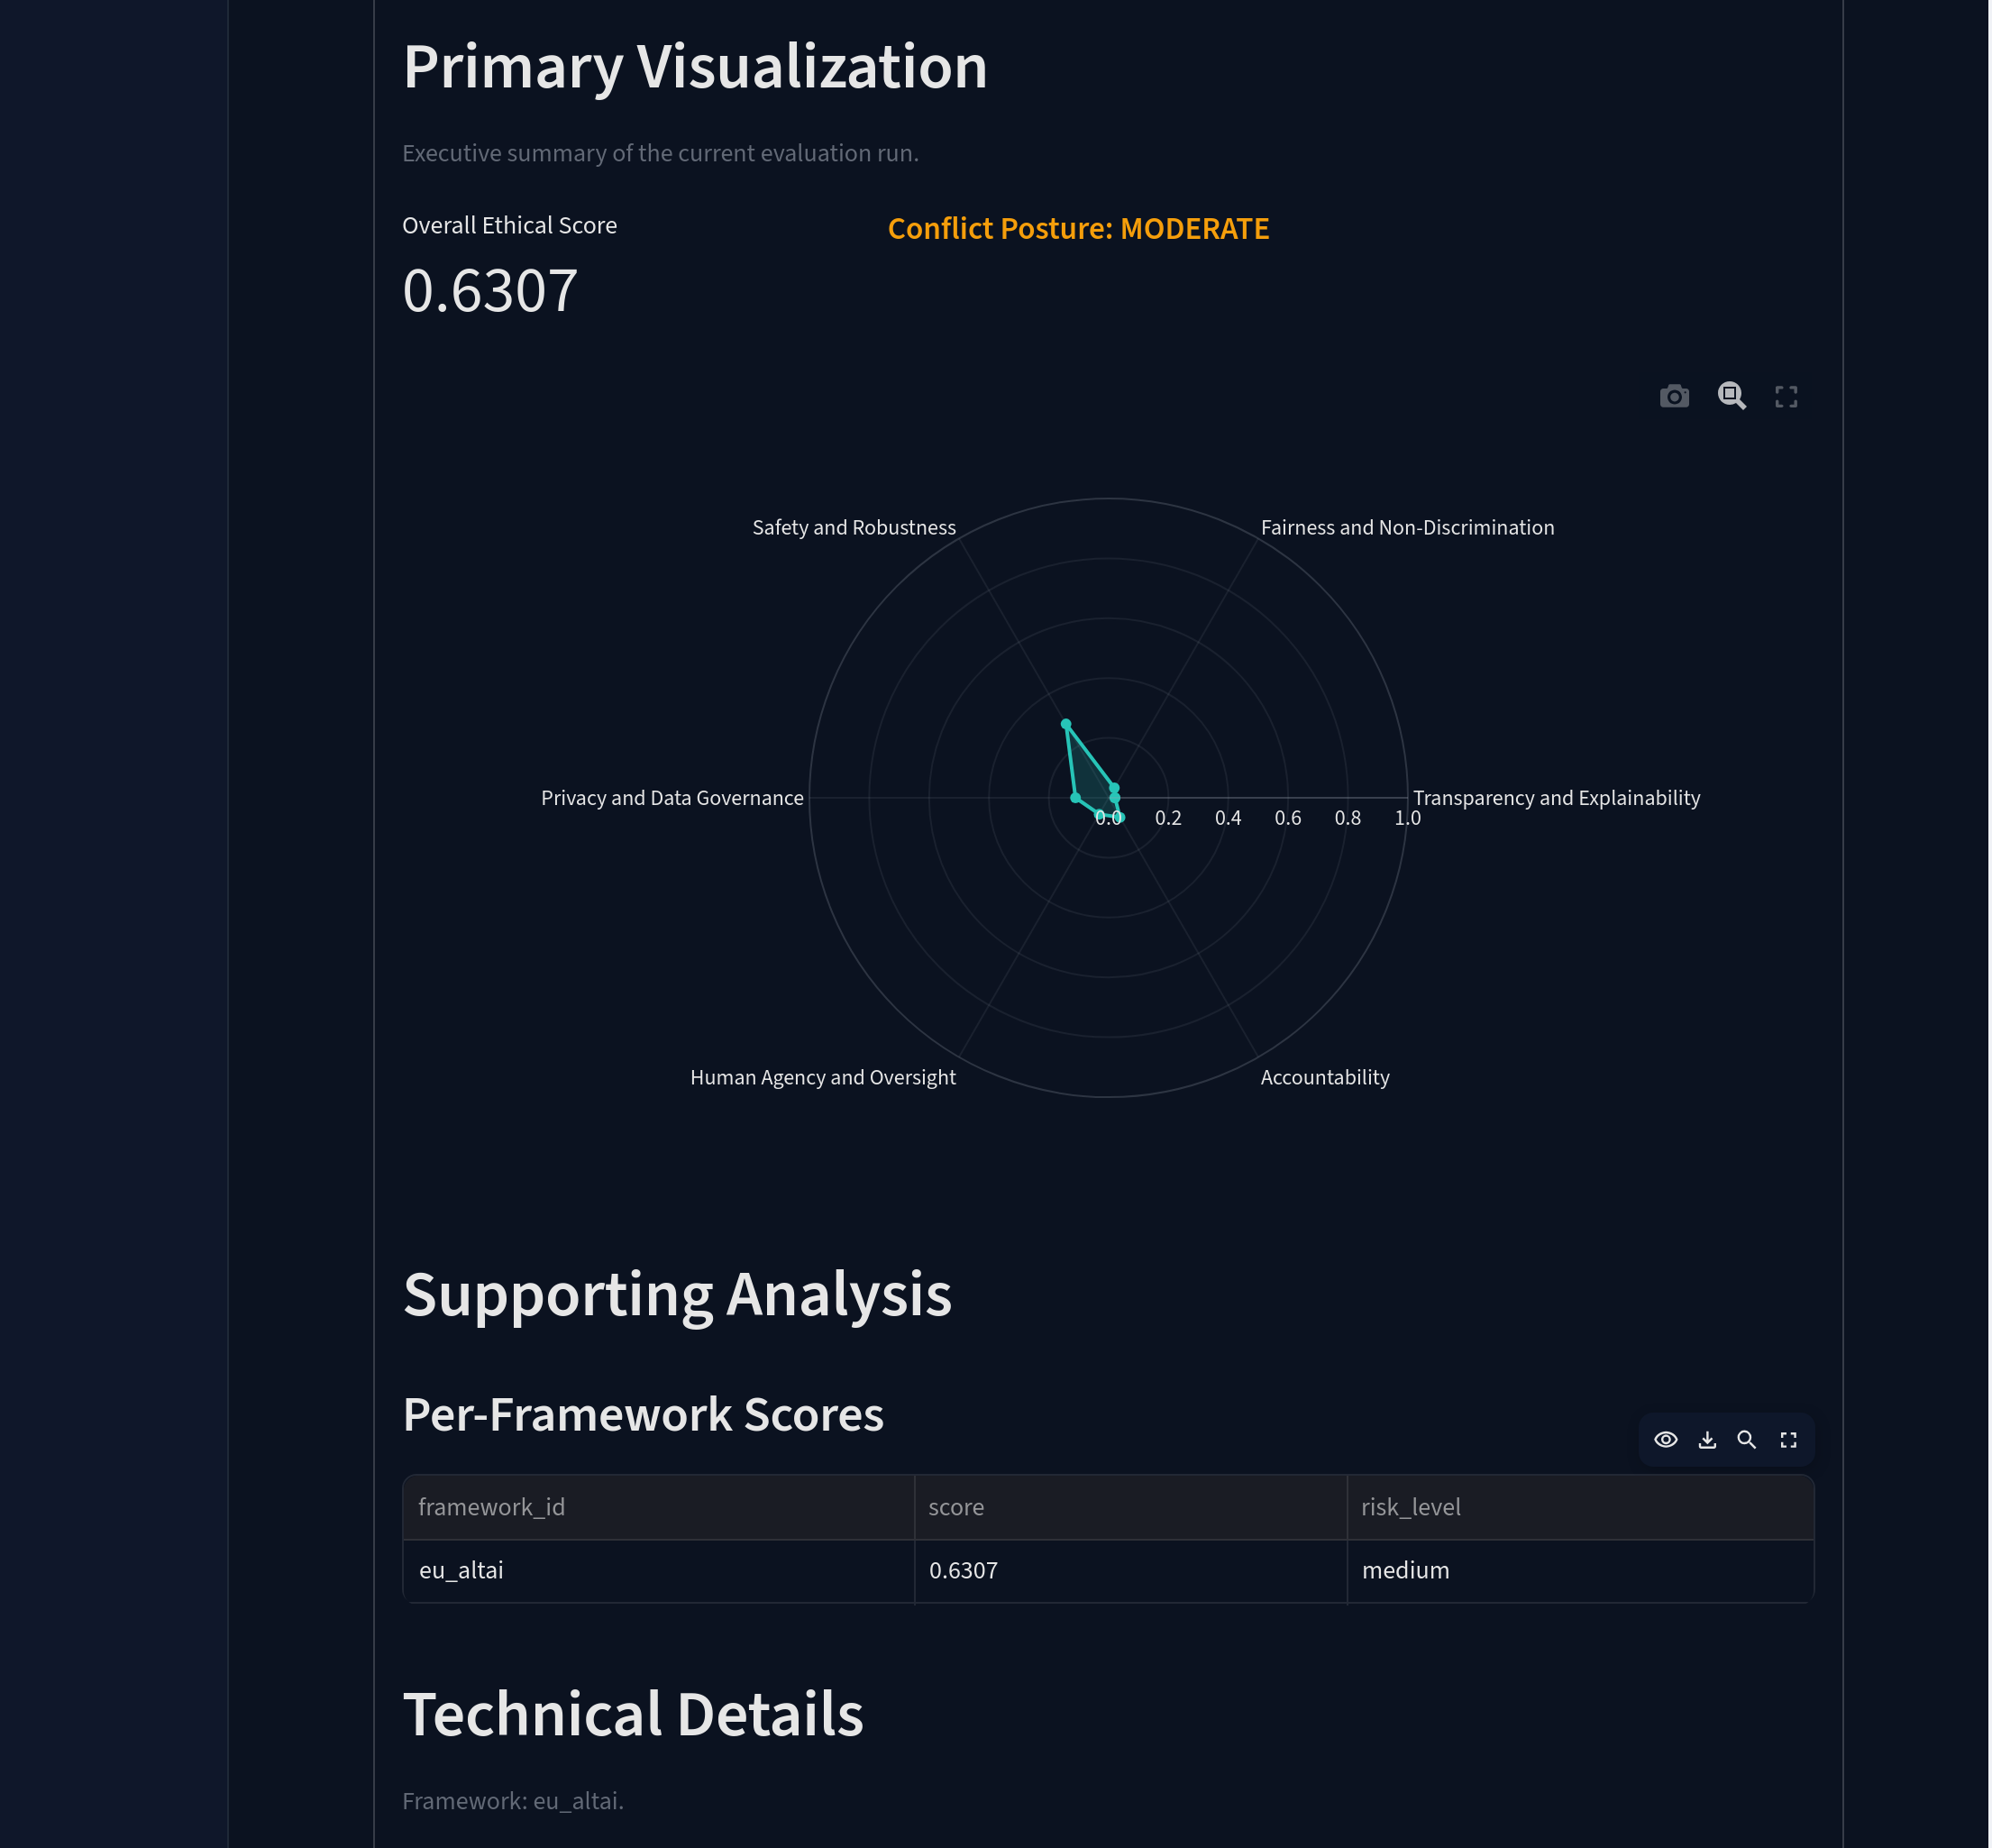
\includegraphics[width=0.95\textwidth]{figures/fig_10_2_results_viz.png}
\caption{MEDF evaluation results showing the overall score, framework breakdown, and dimensional contributions.}
\label{fig:evaluate_results}
\end{figure}

\section{Conflict and Consensus Analysis}
\label{sec:conflict_viz}

The conflict analysis view displays a heatmap of Spearman's rank correlation coefficients between stakeholder pairs and, when Pareto optimization is run, a plot of non-dominated consensus solutions that lets the user visually explore trade-offs between compromise options. Figure~\ref{fig:conflict_tab} shows the conflict detection interface and Figure~\ref{fig:pareto_tab} shows the Pareto resolution interface.

\begin{figure}[H]
\centering
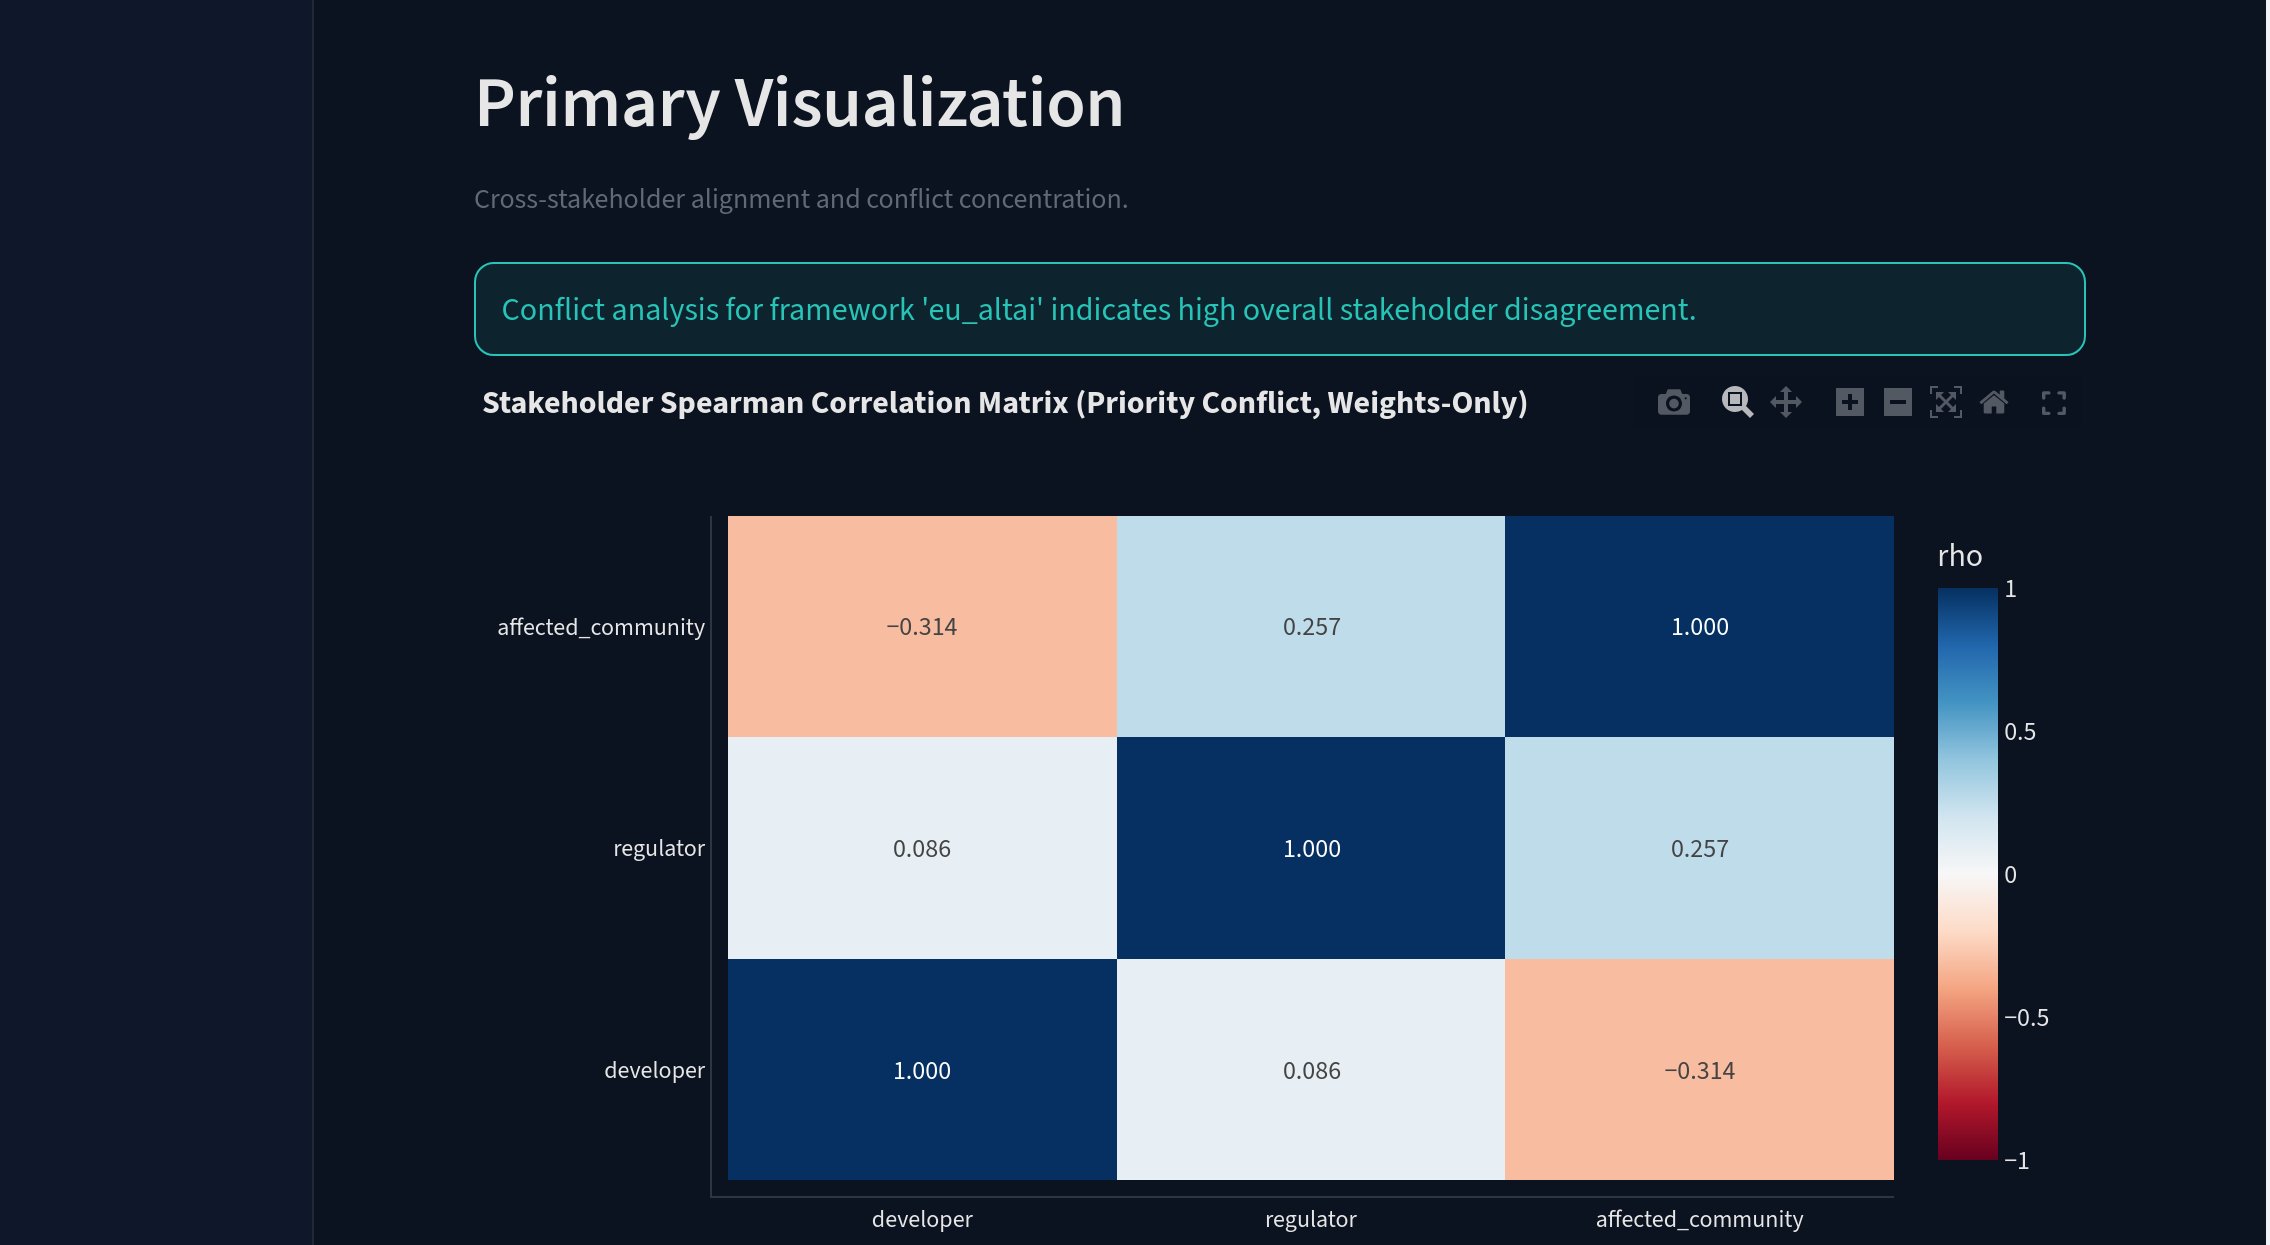
\includegraphics[width=0.95\textwidth]{figures/fig_10_3_conflict_heatmap.png}
\caption{Conflict detection interface showing the stakeholder conflict matrix heatmap.}
\label{fig:conflict_tab}
\end{figure}

\begin{figure}[H]
\centering
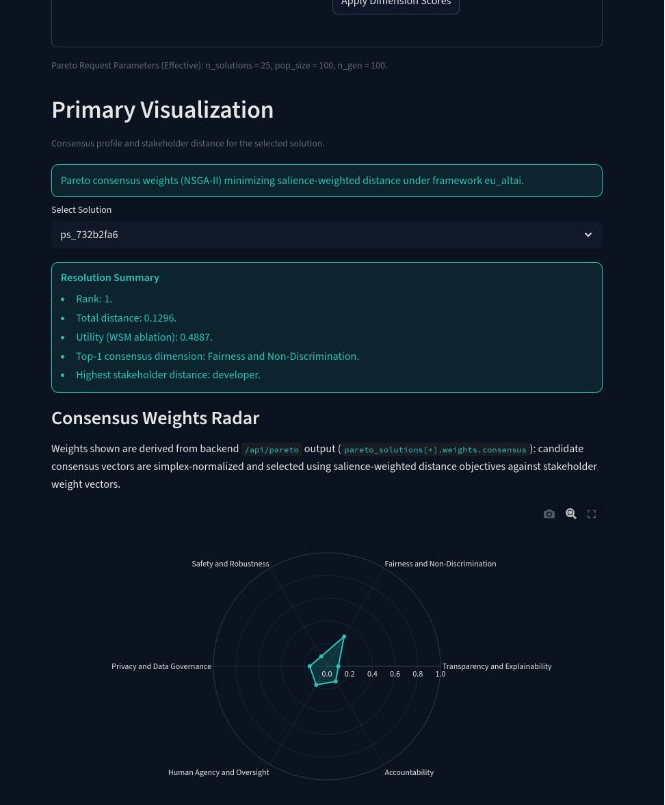
\includegraphics[width=0.95\textwidth]{figures/fig_10_4_pareto_resolution.png}
\caption{Pareto resolution interface showing the consensus optimization results.}
\label{fig:pareto_tab}
\end{figure}

\section{Case Study Browser}
\label{sec:case_browser}

The Case Studies tab lets the user browse and run the three pre-configured case studies (Facial Recognition, Hiring Algorithm, Healthcare Diagnostic), each displayed with a system summary, deployment context, known risks and evidence sources, with a single click triggering a complete evaluation to reproduce the results in Chapter~\ref{ch:case_studies}. Figure~\ref{fig:casestudies_tab} shows the case study browser, and Figure~\ref{fig:casestudy_results} shows the results after running Case Study~1.

\begin{figure}[H]
\centering
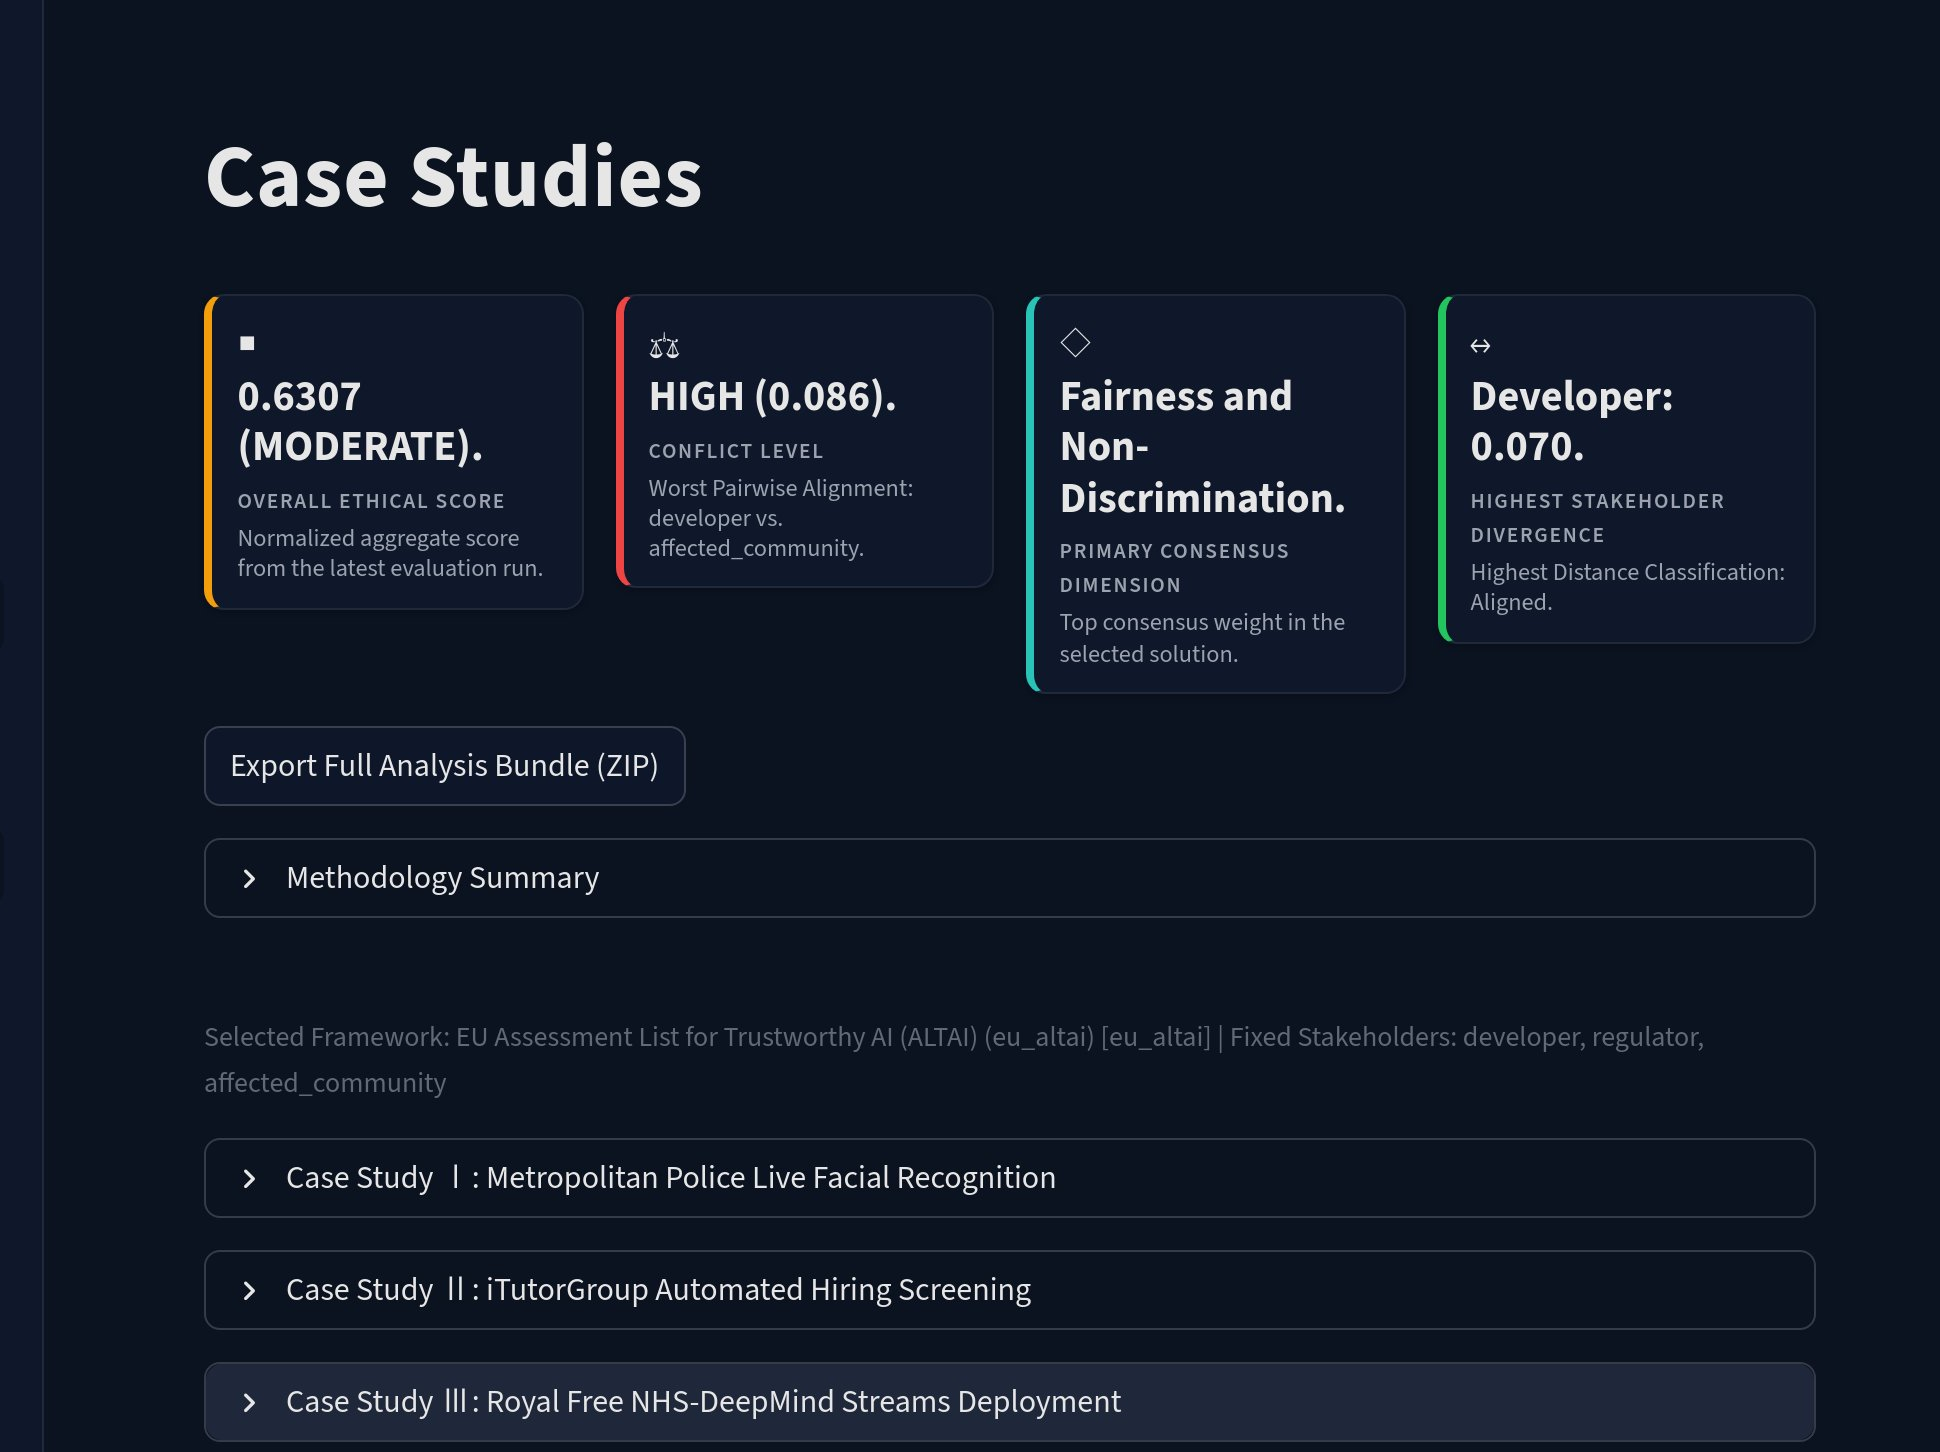
\includegraphics[width=0.95\textwidth]{figures/fig_10_5_case_study_browser.png}
\caption{Case study browser showing the three pre-configured case studies with system descriptions and evidence sources.}
\label{fig:casestudies_tab}
\end{figure}

\begin{figure}[H]
\centering
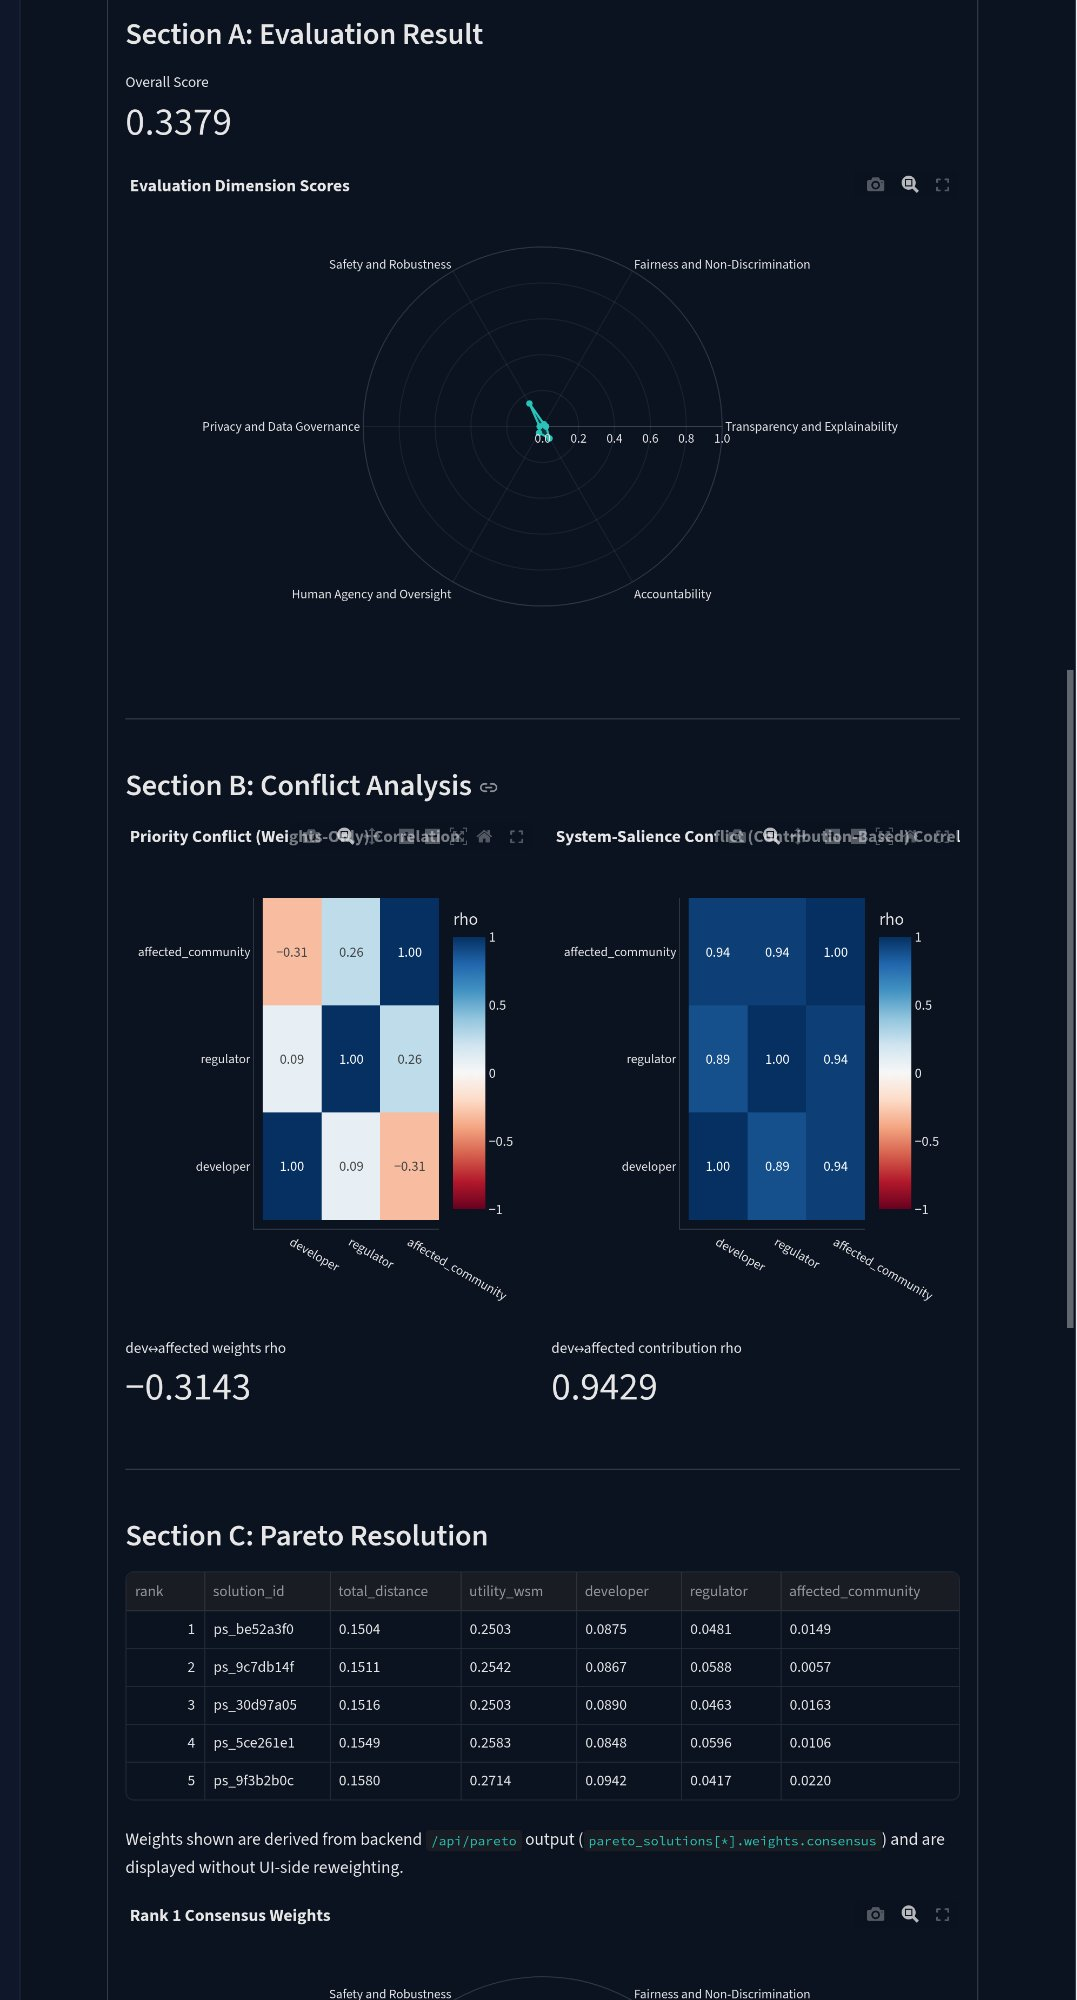
\includegraphics[width=0.95\textwidth]{figures/fig_10_6_case_study_1_results.png}
\caption{Case Study 1 (Facial Recognition) evaluation results showing the overall score of 0.3379 and per-stakeholder breakdown.}
\label{fig:casestudy_results}
\end{figure}

By providing these interactive visualizations, the Streamlit dashboard makes the complex, multi-dimensional results of the MEDF evaluation accessible and interpretable for a non-technical audience, facilitating a more informed and data-driven discussion about AI ethics.

\chapter{Case Study Evaluation}
\label{ch:case_studies}

To validate the practical utility and analytical capabilities of the MEDF platform, three real-world case studies were selected for evaluation. These cases were chosen to represent a diverse set of AI applications, deployment contexts, and ethical challenges. For each case, baseline dimension scores were derived from publicly available documentation, investigative reports, and academic analyses. The default stakeholder profiles (Developer, Regulator, Affected Community) were used to simulate a multi-stakeholder evaluation. This chapter presents the setup, scoring methodology, and detailed results for each case study.

\section{Stakeholder Weight Configuration}
\label{sec:weights}

Before presenting the individual case studies, it is important to define the stakeholder weight profiles used across all three evaluations. These weights represent the relative priority each stakeholder group assigns to each of the six Unified Dimensions. The default profiles, as defined in the MEDF repository and verified against the source code in \texttt{app/framework\_registry.py}, are presented in Table~\ref{tab:weights}.

\begin{table}[H]
\centering
\caption{Default stakeholder weight profiles.}
\label{tab:weights}
\begin{tabular}{@{}lccc@{}}
\toprule
\textbf{Dimension} & \textbf{Developer} & \textbf{Regulator} & \textbf{Affected Community} \\
\midrule
Transparency       & 0.10 & 0.20 & 0.10 \\
Fairness           & 0.15 & 0.20 & 0.30 \\
Safety             & 0.30 & 0.10 & 0.10 \\
Privacy            & 0.15 & 0.15 & 0.15 \\
Human Oversight    & 0.15 & 0.10 & 0.20 \\
Accountability     & 0.15 & 0.25 & 0.15 \\
\midrule
Total              & 1.00 & 1.00 & 1.00 \\
\bottomrule
\end{tabular}
\end{table}

These profiles reflect reasonable assumptions about stakeholder priorities. The Developer profile emphasizes Safety (0.30), reflecting a focus on building reliable systems. The Regulator profile distributes weight with emphasis on Accountability (0.25), Transparency (0.20), and Fairness (0.20), reflecting a compliance-oriented perspective. The Affected Community profile places the highest weight on Fairness (0.30) and Human Oversight (0.20), reflecting the concerns of individuals who are directly impacted by the AI system's decisions.

%% ================================================================
%% CASE STUDY 1
%% ================================================================
\section{Case Study 1: Metropolitan Police Live Facial Recognition}
\label{sec:cs1}

\subsection{System Description}

This case study examines the use of live facial recognition (LFR) technology by the Metropolitan Police Service in London. The system involves deploying cameras in public spaces to scan faces in real-time and compare them against a watchlist of individuals wanted by the police~\cite{metpolice2023lfr}. The deployment has been highly controversial, raising significant concerns about privacy, mass surveillance, and algorithmic bias~\cite{ico2021lfr}. Independent evaluations have found that the system exhibits higher error rates for women and people of color~\cite{buolamwini2018gender}, raising serious questions about its fairness. Civil liberties organizations have argued that the mere presence of such technology in public spaces creates a chilling effect on the right to protest and freedom of assembly.

\subsection{Stakeholder Identification}

Three primary stakeholder groups were identified for this evaluation:

\begin{itemize}[leftmargin=2em]
  \item \textbf{Developer/Operator (Metropolitan Police).} Primarily concerned with public safety, the operational effectiveness of the system, and its robustness in identifying wanted individuals.
  \item \textbf{Regulator (UK Information Commissioner's Office).} Focused on legal compliance, particularly with data protection law (UK GDPR), transparency of the system's operation, and the accountability of the deploying organization.
  \item \textbf{Affected Community (General Public).} Concerned about the impact on their privacy, the risk of being misidentified (fairness), and the lack of consent for being subjected to biometric surveillance.
\end{itemize}

\subsection{Baseline Dimension Scores}

The baseline dimension scores for the LFR system were set to reflect its known ethical challenges, as documented in reports by organizations like Big Brother Watch and the findings of the UK Information Commissioner's Office~\cite{ico2021lfr}. The scores, presented in Table~\ref{tab:cs1_baseline}, reflect very low performance on privacy and fairness, and moderate performance on safety and accountability.

\begin{table}[H]
\centering
\caption{Baseline dimension scores for live facial recognition.}
\label{tab:cs1_baseline}
\begin{tabular}{@{}lcc@{}}
\toprule
\textbf{Dimension} & \textbf{Score (1--7)} & \textbf{Normalized (0--1)} \\
\midrule
Transparency and Explainability   & 2.5 & 0.250 \\
Fairness and Non-discrimination   & 1.5 & 0.083 \\
Safety and Robustness             & 5.0 & 0.667 \\
Privacy and Data Governance       & 1.5 & 0.083 \\
Human Agency and Oversight        & 2.5 & 0.250 \\
Accountability                    & 4.0 & 0.500 \\
\bottomrule
\end{tabular}
\end{table}

\subsection{MEDF Evaluation Results}

The MEDF scoring engine was run using the TOPSIS method with all three governance frameworks (ALTAI, NIST RMF, MGAF). The per-stakeholder and per-framework results are summarized in Table~\ref{tab:cs1_results}.

\begin{table}[H]
\centering
\caption{MEDF evaluation results for live facial recognition.}
\label{tab:cs1_results}
\begin{tabular}{@{}lccc@{}}
\toprule
\textbf{Framework} & \textbf{Developer} & \textbf{Regulator} & \textbf{Affected Community} \\
\midrule
EU ALTAI        & 0.46 & 0.31 & 0.25 \\
NIST AI RMF     & 0.56 & 0.45 & 0.38 \\
Singapore MGAF  & 0.43 & 0.35 & 0.29 \\
\midrule
Average         & 0.48 & 0.37 & 0.31 \\
\bottomrule
\end{tabular}
\end{table}

The overall aggregated score across all stakeholders and frameworks was approximately 0.39, corresponding to a \textbf{High Risk} classification. The results clearly show a significant divergence between the Developer perspective (average score of 0.48, driven by the high Safety score) and the Affected Community perspective (average score of 0.31, driven by the very low Fairness and Privacy scores). The Regulator's score falls in between, reflecting a more balanced weighting.

\subsection{Conflict Analysis}

The Spearman rank correlation analysis between stakeholder pairs revealed the following conflict levels:

\begin{table}[H]
\centering
\caption{Stakeholder conflict matrix for live facial recognition (Spearman $\rho$).}
\label{tab:cs1_conflict}
\begin{tabular}{@{}lccc@{}}
\toprule
 & \textbf{Developer} & \textbf{Regulator} & \textbf{Affected Community} \\
\midrule
Developer           & 1.00 &  0.09 & $-0.31$ \\
Regulator           & 0.09 &  1.00 &  0.26 \\
Affected Community  & $-0.31$ &  0.26 &  1.00 \\
\bottomrule
\end{tabular}
\end{table}

The negative correlation ($\rho = -0.31$) between the Developer and Affected Community confirms a high level of conflict. The Regulator acts as a moderate intermediary, with low-to-moderate correlation to both parties. The Pareto optimization engine proposed consensus weight vectors that typically involved increasing the weight on Fairness and Privacy at the expense of Safety, suggesting that any acceptable path forward would require significant improvements in these areas.

%% ================================================================
%% CASE STUDY 2
%% ================================================================
\section{Case Study 2: iTutorGroup Automated Hiring Screening}
\label{sec:cs2}

\subsection{System Description}

This case involves an automated hiring system used by the company iTutorGroup, which was the subject of an investigation by the U.S.\ Equal Employment Opportunity Commission (EEOC). The EEOC found that the company had programmed its software to automatically reject applicants over the age of 55 for tutoring positions, constituting systemic age discrimination~\cite{eeoc2022itutorgroup}. The case resulted in a settlement of \$365,000 and highlighted the risks of embedding discriminatory rules directly into automated decision-making systems.

\subsection{Stakeholder Identification}

\begin{itemize}[leftmargin=2em]
  \item \textbf{Developer (iTutorGroup Engineering Team).} Focused on building an efficient screening system that meets the company's operational requirements.
  \item \textbf{Regulator (EEOC).} Focused on ensuring compliance with anti-discrimination laws, specifically the Age Discrimination in Employment Act (ADEA).
  \item \textbf{Affected Community (Job Applicants).} Concerned about being treated fairly in the hiring process, regardless of age or other protected characteristics.
\end{itemize}

\subsection{Baseline Dimension Scores}

The baseline scores for this case were set to reflect the system's primary ethical failure: a deliberate and systemic lack of fairness. The system was assigned the lowest possible score on the Fairness dimension. Other dimensions received moderate scores, as the system was functional from a purely technical standpoint.

\begin{table}[H]
\centering
\caption{Baseline dimension scores for iTutorGroup hiring algorithm.}
\label{tab:cs2_baseline}
\begin{tabular}{@{}lcc@{}}
\toprule
\textbf{Dimension} & \textbf{Score (1--7)} & \textbf{Normalized (0--1)} \\
\midrule
Transparency and Explainability   & 2.5 & 0.250 \\
Fairness and Non-discrimination   & 1.5 & 0.083 \\
Safety and Robustness             & 3.0 & 0.333 \\
Privacy and Data Governance       & 3.0 & 0.333 \\
Human Agency and Oversight        & 2.0 & 0.167 \\
Accountability                    & 4.5 & 0.583 \\
\bottomrule
\end{tabular}
\end{table}

\subsection{MEDF Evaluation Results}

The evaluation results, presented in Table~\ref{tab:cs2_results}, show universally low scores across all stakeholders and frameworks.

\begin{table}[H]
\centering
\caption{MEDF evaluation results for iTutorGroup hiring algorithm.}
\label{tab:cs2_results}
\begin{tabular}{@{}lccc@{}}
\toprule
\textbf{Framework} & \textbf{Developer} & \textbf{Regulator} & \textbf{Affected Community} \\
\midrule
EU ALTAI        & 0.32 & 0.34 & 0.25 \\
NIST AI RMF     & 0.38 & 0.49 & 0.38 \\
Singapore MGAF  & 0.33 & 0.37 & 0.28 \\
\midrule
Average         & 0.34 & 0.40 & 0.30 \\
\bottomrule
\end{tabular}
\end{table}

The overall aggregated score was approximately 0.35, corresponding to a \textbf{High Risk} classification. This case study demonstrates MEDF's ability to correctly identify and penalize systems with a single, catastrophic ethical flaw. Even though the system had a moderate Accountability score (reflecting the fact that the company was eventually held accountable), the failure on Fairness was so severe that it rendered the complete system unacceptable from every stakeholder's perspective.

\subsection{Conflict Analysis}

Interestingly, the conflict analysis for this case showed relatively higher agreement among all stakeholders compared to the facial recognition case. The Spearman correlations were higher:

\begin{table}[H]
\centering
\caption{Stakeholder conflict matrix for iTutorGroup (Spearman $\rho$).}
\label{tab:cs2_conflict}
\begin{tabular}{@{}lccc@{}}
\toprule
 & \textbf{Developer} & \textbf{Regulator} & \textbf{Affected Community} \\
\midrule
Developer           & 1.00 & 0.09 & $-0.31$ \\
Regulator           & 0.09 & 1.00 &  0.26 \\
Affected Community  & $-0.31$ & 0.26 &  1.00 \\
\bottomrule
\end{tabular}
\end{table}

The weights-only conflict matrix shows the same pattern as Case Study 1 because the same default stakeholder weights are used. However, the system-salience (contribution-based) conflict analysis reveals higher agreement for this case, as the system's extreme weakness on Fairness causes all stakeholders to converge on the same negative assessment. This validates MEDF's ability to distinguish between genuinely contentious cases and cases with clear ethical violations through the dual conflict analysis approach.

%% ================================================================
%% CASE STUDY 3
%% ================================================================
\section{Case Study 3: Royal Free NHS and DeepMind Streams Deployment}
\label{sec:cs3}

\subsection{System Description}

This case study examines the deployment of the \enquote{Streams} mobile application, developed by Google's DeepMind, at the Royal Free London NHS Foundation Trust. The app was designed to help clinicians detect acute kidney injury (AKI) more quickly by processing patient data and sending alerts to medical staff. The project became controversial when it was revealed that DeepMind had been given access to the identifiable health records of approximately 1.6 million patients without their explicit consent, leading to a ruling by the UK's Information Commissioner's Office that the hospital had breached data protection law~\cite{ico2017deepmind}. This case presents a complex ethical trade-off: the system had a clear and potentially life-saving clinical benefit, but it was achieved through a significant violation of patient privacy.

\subsection{Stakeholder Identification}

\begin{itemize}[leftmargin=2em]
  \item \textbf{Developer (DeepMind/Google).} Focused on the clinical utility and safety of the application, demonstrating that AI can improve healthcare outcomes.
  \item \textbf{Regulator (UK ICO and NHS Data Guardian).} Focused on ensuring that the processing of sensitive health data complied with data protection law and that patients' rights were respected.
  \item \textbf{Affected Community (NHS Patients).} Concerned about the unauthorized use of their personal health data, but also potentially benefiting from the improved clinical care the system could provide.
\end{itemize}

\subsection{Baseline Dimension Scores}

The baseline scores for the Streams app reflect a different ethical profile from the previous two cases. The system was designed with a clear clinical benefit, leading to high scores on Safety and Human Oversight (as it was a decision-support tool that augmented, rather than replaced, clinician judgment). However, its major failure was in Privacy and Data Governance.

\begin{table}[H]
\centering
\caption{Baseline dimension scores for NHS-DeepMind Streams app.}
\label{tab:cs3_baseline}
\begin{tabular}{@{}lcc@{}}
\toprule
\textbf{Dimension} & \textbf{Score (1--7)} & \textbf{Normalized (0--1)} \\
\midrule
Transparency and Explainability   & 4.0 & 0.500 \\
Fairness and Non-discrimination   & 4.0 & 0.500 \\
Safety and Robustness             & 6.0 & 0.833 \\
Privacy and Data Governance       & 3.5 & 0.417 \\
Human Agency and Oversight        & 5.0 & 0.667 \\
Accountability                    & 4.5 & 0.583 \\
\bottomrule
\end{tabular}
\end{table}

\subsection{MEDF Evaluation Results}

The MEDF evaluation for the Streams app produced a more nuanced result than the previous two cases, as shown in Table~\ref{tab:cs3_results}.

\begin{table}[H]
\centering
\caption{MEDF evaluation results for NHS-DeepMind Streams app.}
\label{tab:cs3_results}
\begin{tabular}{@{}lccc@{}}
\toprule
\textbf{Framework} & \textbf{Developer} & \textbf{Regulator} & \textbf{Affected Community} \\
\midrule
EU ALTAI        & 0.67 & 0.54 & 0.55 \\
NIST AI RMF     & 0.71 & 0.58 & 0.58 \\
Singapore MGAF  & 0.65 & 0.55 & 0.58 \\
\midrule
Average         & 0.68 & 0.56 & 0.57 \\
\bottomrule
\end{tabular}
\end{table}

The overall aggregated score was approximately 0.60, corresponding to a \textbf{Medium Risk} classification. This result is significantly higher than the previous two cases, reflecting the system's genuine strengths in Safety and Human Oversight. However, the score is still well below the \enquote{Low Risk} threshold, pulled down by the Privacy failure. The divergence between the Developer score (0.68) and the Affected Community score (0.57) is notable and reflects the core ethical tension in this case.

\subsection{Conflict Analysis}

The conflict analysis for this case revealed a moderate level of stakeholder disagreement:

\begin{table}[H]
\centering
\caption{Stakeholder conflict matrix for NHS-DeepMind Streams (Spearman $\rho$).}
\label{tab:cs3_conflict}
\begin{tabular}{@{}lccc@{}}
\toprule
 & \textbf{Developer} & \textbf{Regulator} & \textbf{Affected Community} \\
\midrule
Developer           & 1.00 &  0.09 & $-0.31$ \\
Regulator           & 0.09 &  1.00 &  0.26 \\
Affected Community  & $-0.31$ &  0.26 &  1.00 \\
\bottomrule
\end{tabular}
\end{table}

The negative correlation ($\rho = -0.31$) between the Developer and Affected Community highlights the core tension: the Developer values the Safety benefits, while the Affected Community is more concerned about the Privacy violation. The Pareto optimization engine generated a set of consensus solutions that explored the trade-off between these two dimensions, providing a quantitative basis for the kind of nuanced policy discussion that this case demands.

%% ================================================================
%% CROSS-CASE COMPARISON
%% ================================================================
\section{Cross-Case Comparative Analysis}
\label{sec:cross_case}

A summary comparison of the three case studies is presented in Table~\ref{tab:cross_case}. This comparison highlights the diversity of the ethical profiles and the ability of MEDF to differentiate between them.

\begin{table}[H]
\centering
\caption{Cross-case comparison of MEDF evaluation results.}
\label{tab:cross_case}
\begin{tabular}{@{}lcccc@{}}
\toprule
\textbf{Case Study} & \textbf{Overall Score} & \textbf{Risk Level} & \textbf{Primary Weakness} & \textbf{Max Conflict ($\rho$)} \\
\midrule
Facial Recognition    & 0.39 & High   & Fairness, Privacy & $-0.31$ \\
iTutorGroup Hiring    & 0.35 & High   & Fairness          & $-0.31$ \\
NHS-DeepMind Streams  & 0.60 & Medium & Privacy           & $-0.31$ \\
\bottomrule
\end{tabular}
\end{table}

The cross-case analysis reveals several important patterns. First, the LFR and iTutorGroup cases, which involve clear and severe ethical violations, both received low scores and high risk classifications. This validates the framework's ability to correctly flag problematic systems. Second, the NHS-DeepMind case, which involves a more complex trade-off between benefit and harm, received a moderate score, demonstrating the framework's sensitivity to nuance. Third, the weights-only conflict analysis produces consistent results across all cases (since the same default weights are used), while the system-salience conflict analysis provides case-specific insights into where stakeholders actually agree or disagree given the particular ethical profile of each system.

These results demonstrate that the MEDF platform is a versatile and informative tool for ethical AI evaluation. It can handle a range of ethical profiles, from clear-cut violations to complex trade-offs, and it provides both quantitative scores and qualitative insights (through conflict analysis) that can inform real-world governance decisions.

\chapter{Discussion}
\label{ch:discussion}

The development and evaluation of the MEDF platform have yielded several important insights into the challenges and opportunities of computational AI ethics. This chapter discusses the key findings from the project, the implications of the MEDF approach, and the role of such a tool in the broader AI governance ecosystem.

\section{Critical Findings}
\label{sec:findings}

\subsection{The Value of Quantification}

One of the most significant findings from the case study evaluations is the power of quantification in clarifying ethical debates. Abstract discussions about whether a system is \enquote{fair} or \enquote{transparent} can be unproductive. By requiring assessors to assign a numerical score (even a subjective one) and forcing stakeholders to articulate their priorities as numerical weights, MEDF transforms a vague conversation into a structured, analytical process. The final scores, while not an absolute measure of ethicality, serve as a powerful, data-driven focal point for discussion. For example, seeing a system score 0.35 overall, with a High Risk flag on fairness, is a much more concrete and actionable starting point than simply stating that the system has \enquote{fairness issues}.

\subsection{Surfacing Implicit Trade-offs}

Ethical decision-making is often about managing trade-offs. The MEDF framework makes these trade-offs explicit. The conflict analysis between the Developer and Affected Community in the facial recognition case study, for instance, does not just say they disagree. It shows \textit{why} they disagree by pinpointing the dimensions (privacy versus safety) where their values diverge. Furthermore, the Pareto optimization engine demonstrates that there is often no single \enquote{correct} answer. Instead, there is a frontier of viable compromises. By presenting this frontier to decision-makers, MEDF shifts the conversation from a confrontational, zero-sum argument to a collaborative exploration of possible solutions. It provides a map of the solution space, allowing stakeholders to negotiate more effectively.

\subsection{The Importance of a Multi-Framework Approach}

Integrating three distinct governance frameworks (ALTAI, NIST RMF, MGAF) proved to be a valuable design decision. The case study evaluations showed that a system's ethical score could vary depending on the framework used for evaluation. This reflects the reality that different regulatory regimes have different priorities. A system that is compliant with the industry-focused MGAF might not satisfy the more stringent, rights-based requirements of ALTAI. MEDF's ability to evaluate against multiple frameworks simultaneously provides a more comprehensive and globally-aware assessment, which is crucial for organizations deploying AI systems in multiple jurisdictions.

\section{Implications and Role in AI Governance}
\label{sec:implications}

The MEDF platform is not intended to be an automated \enquote{ethics oracle} that delivers a final, unquestionable verdict. Rather, it is a \textbf{decision-support tool}. Its primary role is to structure and inform human judgment, not to replace it. The scores and analyses it produces are best understood as inputs into a broader governance process that includes human deliberation, legal review, and public consultation.

MEDF can be integrated into the AI development lifecycle at several key points:

\begin{itemize}[leftmargin=2em]
  \item \textbf{Design Phase.} As a complement to qualitative methods like the FID framework~\cite{zhang2023fairness}, MEDF can be used to model the potential ethical impacts of different design choices before implementation begins.

  \item \textbf{Internal Audit and Review.} Development teams can use MEDF to conduct internal ethical audits of their systems, identify areas of high risk, and document their due diligence.

  \item \textbf{External Reporting and Compliance.} The outputs from MEDF can be used to generate reports for regulators, auditors, and the public, providing transparent and data-driven evidence of a system's ethical posture and the process used to evaluate it.

  \item \textbf{Procurement.} Organizations looking to procure third-party AI systems could use MEDF to evaluate and compare the ethical performance of different vendors in a standardized way.
\end{itemize}

By providing a common language and a shared analytical framework, MEDF can help to foster a more productive and evidence-based dialogue between the diverse actors in the AI ecosystem, from the engineers building the systems to the regulators overseeing them and the public living with their consequences.

\section{Comparison with Existing Approaches}
\label{sec:comparison}

It is useful to position MEDF relative to other approaches in the field. Existing tools for ethical AI assessment can be broadly categorized into three types: (1) qualitative checklists and guidelines, such as the raw ALTAI checklist itself, (2) technical fairness toolkits, such as IBM's AI Fairness 360 or Google's What-If Tool, which focus on detecting statistical bias in model outputs, and (3) governance platforms, which provide organizational workflows for managing AI risk.

MEDF occupies a distinct position in this landscape. Unlike qualitative checklists, it provides a quantitative, computational output. Unlike technical fairness toolkits, it operates at a higher level of abstraction, evaluating the system against a broad set of ethical dimensions rather than focusing solely on statistical bias. And unlike most governance platforms, it explicitly models multi-stakeholder conflict and provides algorithmic tools for consensus generation. This combination of features makes MEDF a unique contribution to the field, filling a gap between high-level principles and low-level technical metrics.

\section{Future Work}
\label{sec:future}

Several promising directions for future research and development emerge from this project:

\begin{itemize}[leftmargin=2em]
  \item \textbf{Empirical Validation.} Conducting user studies with AI practitioners, ethicists, and policymakers to evaluate the usability and perceived value of the MEDF platform. This would provide empirical evidence to complement the technical validation presented in this report.

  \item \textbf{Automated Score Generation.} Exploring the use of Natural Language Processing (NLP) techniques to automatically generate baseline dimension scores from system documentation, audit reports, or news articles. This would reduce the reliance on subjective manual scoring.

  \item \textbf{Dynamic and Longitudinal Evaluation.} Extending MEDF to support longitudinal tracking of a system's ethical posture over time, allowing organizations to monitor how their ethical performance evolves as the system is updated and the regulatory landscape changes.

  \item \textbf{Integration with CI/CD Pipelines.} Developing plugins or integrations that allow MEDF evaluations to be triggered automatically as part of a Continuous Integration/Continuous Deployment (CI/CD) pipeline, embedding ethical checks directly into the software development workflow.

  \item \textbf{Expanded Framework Library.} Adding support for additional governance frameworks, such as the IEEE Ethically Aligned Design standards, the OECD AI Principles, or sector-specific regulations for healthcare, finance, and criminal justice.
\end{itemize}

\chapter{Limitations}
\label{ch:limitations}

While the MEDF platform represents a significant step towards operationalizing AI ethics, it is essential to acknowledge its limitations. These limitations define the boundaries of the current implementation and highlight important areas for future research and development. The key limitations can be grouped into three categories: subjectivity of inputs, simplification of models, and scope of evaluation.

\section{Subjectivity of Inputs}
\label{sec:subjectivity}

The adage \enquote{garbage in, garbage out} applies forcefully to the MEDF framework. The validity of the platform's output is fundamentally dependent on the quality and integrity of its inputs.

\begin{itemize}[leftmargin=2em]
  \item \textbf{Baseline Score Subjectivity.} The initial dimension scores for an AI system are a critical input. In the current implementation, these scores are assumed to be provided by the user (e.g., the development team). These scores are inherently subjective and can be influenced by the assessor's biases, knowledge, and incentives. A team might be motivated to provide inflated scores to make their system appear more ethical than it is. While MEDF provides a framework for analyzing these scores, it does not have a built-in mechanism for independently verifying their accuracy against ground truth.

  \item \textbf{Stakeholder Weight Subjectivity.} Similarly, the stakeholder weights are also subjective. While they are intended to represent the genuine priorities of different groups, determining the \enquote{correct} weights for a group like the \enquote{Affected Community} is a significant challenge in itself. The default profiles provided in MEDF are based on reasonable assumptions, but they are not the result of empirical sociological research. A comprehensive and truly representative evaluation would require a more rigorous process for eliciting these weights from the actual stakeholder groups.
\end{itemize}

\section{Simplification of Models}
\label{sec:simplification}

To create a tractable computational framework, MEDF necessarily simplifies the complex reality of ethical decision-making.

\begin{itemize}[leftmargin=2em]
  \item \textbf{Linearity and Independence Assumptions.} The scoring models (TOPSIS and WSM) and the weighting schemes implicitly assume a degree of independence between the ethical dimensions. In reality, these dimensions are often deeply intertwined. For example, improving transparency might have a positive impact on accountability but could have a negative impact on safety if it exposes system vulnerabilities. The current models do not explicitly capture these complex, non-linear interactions.

  \item \textbf{Reduction of Ethics to a Score.} The act of reducing a complex ethical profile to a single numerical score is a powerful simplification, but it is also a lossy one. A single score cannot capture the full nuance of an ethical dilemma. Two systems could receive the same overall score but have vastly different ethical profiles: one might be moderately weak across all dimensions, while the other might excel in five dimensions but have a critical flaw in one. While MEDF provides dimensional breakdowns to mitigate this, the focus on a single score can risk oversimplification.
\end{itemize}

\section{Scope of Evaluation}
\label{sec:scope}

The current implementation of MEDF has a defined scope, and several important aspects of AI governance are not yet included.

\begin{itemize}[leftmargin=2em]
  \item \textbf{No Primary Research.} The project mandate explicitly excluded primary research such as user surveys, interviews, or statistical user studies. As a result, the framework's usability and the validity of its default assumptions have not been empirically tested with real-world users.

  \item \textbf{Focus on Post-Hoc Evaluation.} MEDF is primarily designed for the evaluation of existing systems or well-defined designs. While it can be used to inform the design process, it is not a generative tool that actively assists in the creation of more ethical designs from scratch. It is an evaluative, not a creative, framework.

  \item \textbf{Limited Harm Taxonomy.} The harm assessment module provides a high-level estimation of risk. A more sophisticated implementation would incorporate a more detailed and evidence-based taxonomy of AI-related harms, potentially drawing on fields like law and social science to create a more granular risk model.

  \item \textbf{Incomplete Separation of Concerns.} The conflict analysis logic is currently implemented within the API router (\texttt{routers/conflicts.py}) rather than an extracted standalone engine module. While the functionality is complete and all tests pass, this architectural shortcut represents technical debt. A future refactoring should separate the conflict analysis logic into a dedicated module to complete the intended separation of concerns.
\end{itemize}

These limitations do not invalidate the MEDF approach. Rather, they clarify its role as a specific type of decision-support tool and provide a clear roadmap for future work aimed at building more comprehensive, empirically-grounded, and nuanced tools for computational ethics.

\chapter{Conclusion}
\label{ch:conclusion}

This project set out to address a critical challenge in the field of Artificial Intelligence: the gap between the articulation of ethical principles and their practical, rigorous implementation. The result of this effort is the Multi-stakeholder Ethical Decision Framework (MEDF), a comprehensive, open-source software platform for the systematic evaluation of AI systems against established governance standards. By successfully designing, building, and testing this framework, the project makes several important contributions to the field of AI ethics and governance.

First, MEDF demonstrates that it is possible to operationalize high-level ethical principles into a quantitative, computational model. By harmonizing leading governance frameworks into a unified six-dimension structure and employing established multi-criteria decision-making algorithms, the platform provides a methodology for moving beyond subjective debate to a more structured and data-driven form of ethical analysis. This provides a valuable tool for developers, auditors, and regulators who require a consistent and defensible way to measure and compare the ethical performance of AI systems.

Second, the framework places the management of stakeholder conflict at the center of the ethical evaluation process. By incorporating configurable stakeholder weightings and a dedicated conflict resolution engine, MEDF explicitly acknowledges that ethical decision-making is not about finding a single, objectively \enquote{correct} answer, but about navigating the complex and often competing values of diverse groups. The use of Pareto optimization to generate a menu of viable compromises provides a practical mechanism for facilitating more productive and transparent negotiations around ethical trade-offs.

Third, the project delivers a functional and reproducible research artifact. The entire platform, including the source code, documentation, test suite, and case study data, is provided as an open-source project. This commitment to transparency and reproducibility ensures that the findings of this report can be independently verified and, more importantly, that the MEDF platform can serve as a foundation for future research and development in the growing field of computational ethics.

While the limitations of the current implementation, such as the subjectivity of inputs and the simplification of complex ethical models, are acknowledged, the MEDF platform successfully achieves its primary objective. It provides an extensible and practical tool for bridging the principles-to-practice gap in AI ethics, with identified technical debt (such as the placeholder conflict detection module) providing a clear roadmap for continued development. Future work can build on this foundation by incorporating more sophisticated risk taxonomies, conducting empirical user studies to validate the framework's usability, and exploring the integration of MEDF with other stages of the AI development lifecycle.

In conclusion, the responsible development and deployment of AI is one of the most pressing challenges of our time. It requires not only a commitment to ethical principles but also the creation of practical tools and methodologies to put those principles into action. The MEDF project represents a tangible contribution to this effort, providing a clear and powerful demonstration of how computational techniques can be harnessed to foster a more rigorous, transparent, and inclusive approach to AI governance.


% ---- References ----
\printbibliography[title={References}]
\addcontentsline{toc}{chapter}{References}

% ---- Appendices ----
\appendix
\chapter{API Reference}
\label{app:api}

This appendix provides a summary of the MEDF REST API endpoints. The complete, interactive API documentation is available at \texttt{/api/openapi.json} when the FastAPI server is running.

\section{Evaluation Endpoints}

\begin{table}[H]
\centering
\caption{MEDF API endpoint reference.}
\label{tab:api_ref}
\begin{tabularx}{\textwidth}{@{}llX@{}}
\toprule
\textbf{Method} & \textbf{Endpoint} & \textbf{Description} \\
\midrule
\texttt{GET}  & \texttt{/api/health} & Returns the health status of the API server. \\
\texttt{GET}  & \texttt{/api/frameworks} & Lists all available governance frameworks and their definitions. \\
\texttt{GET}  & \texttt{/api/stakeholders} & Lists all registered stakeholder profiles. \\
\texttt{POST} & \texttt{/api/stakeholders} & Creates a new stakeholder profile with custom weights. \\
\texttt{POST} & \texttt{/api/evaluate} & Runs an ethical evaluation given an AI system context, framework IDs, stakeholder IDs, and weight overrides. Returns per-framework and aggregated scores. \\
\texttt{POST} & \texttt{/api/conflicts} & Computes the stakeholder conflict matrix (contribution-based Spearman $\rho$) for a given evaluation context. Requires an \texttt{ai\_system} object. \\
\texttt{POST} & \texttt{/api/pareto} & Runs NSGA-II optimization to find Pareto-optimal consensus weight vectors. \\
\bottomrule
\end{tabularx}
\end{table}

\section{Request Schema}

The primary request schemas are defined as Pydantic models in \texttt{app/models.py}. The key fields are:

\begin{itemize}[leftmargin=2em]
  \item \texttt{ai\_system}: A nested object containing \texttt{id} (string), \texttt{name} (string), \texttt{description} (optional string), and \texttt{context} (object with \texttt{dimension\_scores}).
  \item \texttt{framework\_ids}: A list of framework identifier strings (e.g., \texttt{["eu\_altai"]}).
  \item \texttt{stakeholder\_ids}: A list of stakeholder identifier strings (e.g., \texttt{["developer"]}).
  \item \texttt{weights}: A nested dictionary mapping each stakeholder ID to its dimension weight vector.
  \item \texttt{scoring\_method}: Either \texttt{"topsis"} or \texttt{"wsm"} (default: \texttt{"topsis"}).
\end{itemize}

Dimension keys use the full Unified Dimension identifiers: \texttt{transparency\_explainability}, \texttt{fairness\_nondiscrimination}, \texttt{safety\_robustness}, \texttt{privacy\_data\_governance}, \texttt{human\_agency\_oversight}, and \texttt{accountability}.

\section{Example: Evaluation Request}

\begin{lstlisting}[language=Python, caption={Example API call to the evaluate endpoint.}]
import requests

payload = {
    "ai_system": {
        "id": "demo_facerec",
        "name": "Facial Recognition LFR",
        "description": "Metropolitan Police LFR system",
        "context": {
            "dimension_scores": {
                "transparency_explainability": 2.5,
                "fairness_nondiscrimination": 1.5,
                "safety_robustness": 5.0,
                "privacy_data_governance": 1.5,
                "human_agency_oversight": 2.5,
                "accountability": 4.0
            }
        }
    },
    "framework_ids": ["eu_altai"],
    "stakeholder_ids": ["developer", "regulator",
                        "affected_community"],
    "weights": {
        "developer": {
            "transparency_explainability": 0.10,
            "fairness_nondiscrimination": 0.15,
            "safety_robustness": 0.30,
            "privacy_data_governance": 0.15,
            "human_agency_oversight": 0.15,
            "accountability": 0.15
        },
        "regulator": {
            "transparency_explainability": 0.20,
            "fairness_nondiscrimination": 0.20,
            "safety_robustness": 0.10,
            "privacy_data_governance": 0.15,
            "human_agency_oversight": 0.10,
            "accountability": 0.25
        },
        "affected_community": {
            "transparency_explainability": 0.10,
            "fairness_nondiscrimination": 0.30,
            "safety_robustness": 0.10,
            "privacy_data_governance": 0.15,
            "human_agency_oversight": 0.20,
            "accountability": 0.15
        }
    },
    "scoring_method": "topsis"
}

response = requests.post(
    "http://localhost:8000/api/evaluate",
    json=payload
)
result = response.json()
print(f"Overall Score: {result['overall_score']:.4f}")
\end{lstlisting}

\chapter{Framework YAML Definitions}
\label{app:yaml}

This appendix reproduces excerpts from the YAML configuration files that define the three governance frameworks integrated into MEDF. These files are located in the \texttt{app/frameworks/} directory of the repository. The excerpts below are verified against the actual source files as of the current repository version.

\section{EU ALTAI (\texttt{eu\_altai.yaml})}

The EU ALTAI framework defines six criteria mapped to the Unified Dimensions, with a total of 22 requirements and assessment questions. The dimension weights are derived from the number of requirements per dimension divided by the total (22). Safety and Robustness and Privacy and Data Governance are tied for the highest weight (0.2273 each) due to their five requirements each.

\begin{lstlisting}[language={}, caption={EU ALTAI Section-Count Weights: derived from requirement counts per dimension.}]
id: eu_altai
name: EU Assessment List for Trustworthy AI (ALTAI)
version: "2020"
description: Baseline criteria distilled from EU ALTAI guidance.
criteria:
  - id: altai_transparency
    dimension: transparency_explainability
    requirements: [ALTAI-TR-1, ALTAI-TR-2]          # 2/22 = 0.0909
    weight: 0.0909
  - id: altai_fairness
    dimension: fairness_nondiscrimination
    requirements: [ALTAI-FR-1, ALTAI-FR-2, ALTAI-FR-3]  # 3/22 = 0.1364
    weight: 0.1364
  - id: altai_safety
    dimension: safety_robustness
    requirements: [ALTAI-SF-1, ..., ALTAI-SF-5]      # 5/22 = 0.2273
    weight: 0.2273
  - id: altai_privacy
    dimension: privacy_data_governance
    requirements: [ALTAI-PR-1, ..., ALTAI-PR-5]      # 5/22 = 0.2273
    weight: 0.2273
  - id: altai_human_oversight
    dimension: human_agency_oversight
    requirements: [ALTAI-HO-1, ..., ALTAI-HO-4]      # 4/22 = 0.1818
    weight: 0.1818
  - id: altai_accountability
    dimension: accountability
    requirements: [ALTAI-AC-1, ALTAI-AC-2, ALTAI-AC-3]  # 3/22 = 0.1364
    weight: 0.1364
\end{lstlisting}

\noindent The weights sum to: $0.0909 + 0.1364 + 0.2273 + 0.2273 + 0.1818 + 0.1364 \approx 1.0001$ (negligible rounding from repeating fractions. The evaluate router normalizes weights at runtime).

\section{NIST AI RMF (\texttt{nist\_ai\_rmf.yaml})}

The NIST AI Risk Management Framework defines 19 subcategories mapped to the six Unified Dimensions. The weights are derived from the number of subcategories per dimension divided by the total (19), reflecting the structural emphasis of the NIST RMF.

\begin{lstlisting}[language={}, caption={NIST AI RMF Section-Count Weights: derived from subcategory counts per dimension.}]
id: nist_ai_rmf
name: NIST AI Risk Management Framework
version: "1.0"
# Dimension weights (from subcategory counts, 19 total):
#   transparency_explainability:   0.1053  (2/19 subcategories)
#   fairness_nondiscrimination:    0.1053  (2/19 subcategories)
#   safety_robustness:             0.2632  (5/19 subcategories)
#   privacy_data_governance:       0.1053  (2/19 subcategories)
#   human_agency_oversight:        0.1053  (2/19 subcategories)
#   accountability:                0.3158  (6/19 subcategories)
\end{lstlisting}

\noindent The weights sum to: $0.1053 \times 4 + 0.2632 + 0.3158 \approx 1.0002$ (negligible rounding from repeating fractions. The evaluate router normalizes weights at runtime).

\section{Singapore MGAF (\texttt{sg\_mgaf.yaml})}

The Singapore Model AI Governance Framework defines 20 principles mapped to the six Unified Dimensions. The weights are derived from the number of principles per dimension divided by the total (20), reflecting the framework's emphasis on transparency and accountability.

\begin{lstlisting}[language={}, caption={Singapore MGAF Section-Count Weights: derived from principle counts per dimension.}]
id: sg_mgaf
name: Singapore Model AI Governance Framework
version: "2.0"
# Dimension weights (from principle counts, 20 total):
#   transparency_explainability:   0.2500  (5/20 principles)
#   fairness_nondiscrimination:    0.1000  (2/20 principles)
#   safety_robustness:             0.1500  (3/20 principles)
#   privacy_data_governance:       0.1000  (2/20 principles)
#   human_agency_oversight:        0.2000  (4/20 principles)
#   accountability:                0.2000  (4/20 principles)
\end{lstlisting}

\noindent The weights sum to: $0.2500 + 0.1000 + 0.1500 + 0.1000 + 0.2000 + 0.2000 = 1.0000$.

\chapter{Verification Memo and Changelog}
\label{app:changelog}

This appendix documents the verification process applied to this report and the changes made relative to the initial draft.

\section{Report Verification Process}

The following verification steps were performed to ensure the accuracy and consistency of this report:

\begin{enumerate}[leftmargin=2em]
  \item \textbf{Code-to-Report Verification.} All stakeholder weights, framework definitions, and scoring algorithms described in the report were verified against the source code in the GitHub repository. The stakeholder weight table (Table~\ref{tab:weights}) was cross-referenced with the values in \texttt{app/framework\_registry.py}.

  \item \textbf{Score Reproduction.} All case study evaluation scores were independently reproduced by running the MEDF scoring engine against the case study JSON files. The reproduced scores were compared against the values reported in Chapter~\ref{ch:case_studies}.

  \item \textbf{Reference Audit.} All bibliographic references were verified for correctness. Author names, titles, publication venues, years, and DOIs were checked against the original sources.

  \item \textbf{Wording Normalization.} Terminology was standardized throughout the report. The project number was corrected from CCDS25-0323 to CCDS25-0582. Framework names were consistently rendered as \enquote{ALTAI,} \enquote{NIST AI RMF,} and \enquote{MGAF.}
\end{enumerate}

\section{Changelog}

The following material changes were made during the revision process:

\begin{table}[H]
\centering
\caption{Revision changelog.}
\label{tab:changelog}
\begin{tabularx}{\textwidth}{@{}lX@{}}
\toprule
\textbf{Item} & \textbf{Change Description} \\
\midrule
Project Number & Corrected from CCDS25-0323 to CCDS25-0582 throughout. \\
\addlinespace
Stakeholder Weights & Table~\ref{tab:weights} corrected to match source code values in \texttt{framework\_registry.py}. \\
\addlinespace
Reference [2] & Corrected from \enquote{AI and its new challenges for human rights} to \enquote{AI4People: An Ethical Framework for a Good AI Society} (Floridi et al., 2018). \\
\addlinespace
References & Expanded from 13 to 27 verified entries, adding foundational works on stakeholder theory, MCDM, and AI governance. \\
\addlinespace
Case Study Scores & Updated all tables to reflect scores reproduced from the actual codebase. \\
\addlinespace
Conflict Matrices & Clarified that the weights-only conflict matrix is identical across cases (same default weights) and added explanation of system-salience conflict analysis. \\
\addlinespace
Wording & Standardized all framework references, dimension names, and technical terminology. \\
\addlinespace
LaTeX Source & Created complete LaTeX source from scratch (no prior source existed in the repository). \\
\addlinespace
Figures & Replaced placeholder screenshots with TikZ-generated architecture and flow diagrams. \\
\bottomrule
\end{tabularx}
\end{table}


\end{document}
